\documentclass[twoside,openright]{book}
\usepackage{ctex}

\usepackage{amsmath,amssymb,mathtools}
\usepackage{ntheorem}
\usepackage[twoside,top=2.5cm,bottom=2.5cm,left=2.5cm,right=5cm,a4paper,marginparwidth=4cm,marginparsep=0.5cm]{geometry}
\usepackage{physics}
\usepackage{graphicx}
\usepackage{booktabs}
\usepackage{subfigure}
\usepackage{float}
\usepackage{mathrsfs}
\usepackage[colorlinks,linkcolor=blue]{hyperref}
\usepackage{tkz-euclide}
\usepackage{tkz-base}
\usetikzlibrary{math,arrows,backgrounds,scopes,plotmarks,shapes,calc,decorations.pathmorphing,shadows, positioning,fit,petri,intersections,through,backgrounds, shapes.geometric,topaths,automata,mindmap,folding,calendar,chains,circuits,circuits.ee.IEC}
\usetkzobj{all}
\makeatletter
\global\let\tikz@ensure@dollar@catcode=\relax
\makeatother
\usepackage{calc,pifont}
\newcommand\maincolor{cyan}
\usepackage{fancyhdr}
\newcommand\lwidth{17}
\pagestyle{fancy}
%\fancyfoot[r]{\thepage}
\newcommand{\X}{\phantom{X}}


\makeatletter 
\newcommand\figcaption{\def\@captype{figure}\caption} 
\newcommand\tabcaption{\def\@captype{table}\caption} 
\makeatother

\usepackage{caption2}
 \captionsetup{font=footnotesize}
\usepackage{wrapfig}
\usepackage{verbatim}
\usepackage{slashed} 
\usepackage{appendix} 
\usepackage{pdfpages}
\usepackage{wasysym}
\usepackage{setspace}
\usepackage{siunitx}
\usepackage{booktabs}
\usepackage{tagging}
\usepackage{multicol}
%\usepackage{frame}
\usepackage{tabu}
\usepackage{longtable}
\graphicspath{{problem/image/}}

%%%%%%%%%%%%%%%边框文字
\usepackage[explicit]{titlesec}
\usepackage{lmodern}
\usepackage[many]{tcolorbox}
\tcbuselibrary{skins,breakable}
\tcbuselibrary{theorems}


\usepackage{CJKnumb}
\newcommand{\formatsubsection}[1]{
	{\color{\maincolor}\ding{113}\kern0.5em\relax\bf #1}
}
\titleformat{\subsection}[hang]
{}
{}
{0em}
{\formatsubsection{#1}}
\newcommand{\stitle}[1]{\subsection{#1}\label{#1}}



%\theoremstyle{break}
\theorembodyfont{\small}
\theoremindent1cm
\theoremsymbol{\ensuremath{\ast}}
\theoremseparator{}

\newcommand{\formatsection}[1]{
	\begin{center}\begin{tikzpicture}
		\filldraw[draw=\maincolor,fill=\maincolor](0,-.4)--(0,.3)--(.3,.6)--(\lwidth-3.5,.6)--(\lwidth-3.5,-.4)--(0,-.4);
		\node [anchor=west] at(1,.1){\large \color{white} #1};
		\end{tikzpicture}\end{center}
}
\titleformat{\section}[hang]
{\usefont{T1}{qhv}{b}{n}}
{}
{0em}
{\formatsection{#1}}


\newenvironment{post-problem}{
	\newpage\section*{课后练习}
%	\begin{multicols}{2}
	\linespread{1}}{\linespread{1}}
%	\end{multicols}}

\newcounter{example}[chapter]
\newenvironment{example}[1][]{\refstepcounter{example}\par\medskip
	\textbf{\thechapter.\theexample #1} \rmfamily}{\medskip}
%\newtheorem{example}{}[chapter]

\newenvironment{problemfig}{\begin{center}}{ \end{center}}



%\newtcbtheorem[number within=chapter]{eg}{例}
%{breakable,colback=blue!2,colframe=green!25!black,fonttitle=\bfseries,fontupper=\small\CTEXindent,before skip=5mm,code={\singlespacing}}{exa}
\newtcbtheorem[number within=chapter]{app}{例}
{breakable,colback=blue!2,colframe=blue!35!black,fonttitle=\bfseries,fontupper=\small\CTEXindent,fontlower=\small\CTEXindent}{app}

\definecolor{titlebgdark}{RGB}{0,163,243}
\definecolor{titlebglight}{RGB}{191,233,251}


\graphicspath{{image/}} % Specifies the directory where pictures are stored
\renewcommand{\vec}[1]{\vb*{#1}}

\newcommand{\crp}[2]{\vec{#1}\times\vec{#2}}
\newcommand{\dotp}[2]{\vec{#1}\cdot\vec{#2}}
\newcommand{\Ga}[2]{\Gamma^{#1}_{#2}}
\renewcommand{\pb}[2]{\left[{#1},{#2}  \right]_{P.B.}}
\renewcommand{\op}[1]{\^{#1}}
\newcommand{\sch}{Schr\"{o}dinger}
\newcommand{\roma}[1]{\uppercase\expandafter{\romannumeral#1}}
\newcommand{\const}{\text{const.}}
\newcommand{\vdw}{Van der Walls}
\renewcommand{\deg}[1]{#1^\circ}

%\newcommand{\titleform}{第\thechapter 讲}
%%%%%%%%%%%%%%%%%%%%%%%%%%%%%%%%%%%%%%%%%%%%%% chapter format

\titleformat{\chapter}[display]
{\normalfont\huge\bfseries}
{}
{20pt}
{%
	\begin{tcolorbox}[
		enhanced,
		colback=titlebgdark,
		boxrule=0.25cm,
		colframe=titlebglight,
		arc=0pt,
		outer arc=0pt,
		leftrule=0pt,
		rightrule=0pt,
		fontupper=\color{white}\sffamily\bfseries\huge,
		enlarge left by=-1in-\hoffset-\oddsidemargin,
		enlarge right by=-\paperwidth+1in+\hoffset+\oddsidemargin+\textwidth,
		width=\paperwidth,
		left=1in+\hoffset+\oddsidemargin,
		right=\paperwidth-1in-\hoffset-\oddsidemargin-\textwidth,
		top=0.6cm,
		bottom=0.6cm,
		overlay={
			\node[
			fill=titlebgdark,
			draw=titlebglight,
			line width=0.15cm,
			inner sep=0pt,
			text width=1.7cm,
			minimum height=1.7cm,
			align=center,
			font=\color{white}\sffamily\bfseries\fontsize{30}{36}\selectfont
			]
			(chapname)
			at ([xshift=-4cm]frame.north east)
			{\thechapter};
%			\node[font=\small,anchor=south,inner sep=2pt] at (chapname.north)
%			{\MakeUppercase\chaptertitlename};
		}
		]
		#1
	\end{tcolorbox}%
}
\titleformat{name=\chapter,numberless}[display]
{\normalfont\huge\bfseries}
{}
{20pt}
{%
	\begin{tcolorbox}[
		enhanced,
		colback=titlebgdark,
		boxrule=0.25cm,
		colframe=titlebglight,
		arc=0pt,
		outer arc=0pt,
		remember as=title,
		leftrule=0pt,
		rightrule=0pt,
		fontupper=\color{white}\sffamily\bfseries\huge,
		enlarge left by=-1in-\hoffset-\oddsidemargin,
		enlarge right by=-\paperwidth+1in+\hoffset+\oddsidemargin+\textwidth,
		width=\paperwidth,
		left=1in+\hoffset+\oddsidemargin,
		right=\paperwidth-1in-\hoffset-\oddsidemargin-\textwidth,
		top=0.6cm,
		bottom=0.6cm,
		]
		#1
	\end{tcolorbox}%
}
\titlespacing*{\chapter}
{0pt}{0pt}{40pt}
\makeatother

%%%%%%%%%%%%%%%%%%%%%%%%%%%%%%%%%%%%%%%%%%%%

\fancyfoot[c]{}
\renewcommand{\chaptermark}[1]{\markboth{#1}{}}
\fancyfoot[LE,RO]{\begin{tikzpicture}[baseline, every node/.style={minimum size=8mm, anchor=base}]
	\path node at (0,0) [shape=circle, fill=\maincolor!20] (0,0) {\X}
	node at (.8,0) [shape=circle, fill=\maincolor!60] (0,0) {\X}
	node at (1.6,0) [shape=circle, fill=\maincolor] (0,0) { \color{white}\thepage};\end{tikzpicture}}
\fancyhead[L]{\small\it\color{\maincolor}高一$ \cdot $第\thechapter 讲}

\rhead{\small\it\color{\maincolor}\leftmark}










\includeonly{chapter/newton}









\begin{document}
\usetag{student}
\usetag{answer}
\usetag{analysis}

% !TEX root = ../zz-lecture.tex


\chapter{运动学,导数}

高中课程的起始阶段我们就学习了运动学的内容,研究了描述运动的基本物理量、图象、以及匀变速直线运动规律。在这个模块中我们主要介绍相对运动和运动关联的内容。

\stitle{相对运动}

一个物体的运动需要在某个确定的参考系中进行描述,显然,在不同参考系中对同一运动的描述往往是不同的,这就是运动的相对性。例如,古人在有关天体运动的研究中存在地心说和日心说两种对立的学说,日心说认为太阳是宇宙的中心,地心说认为地球是宇宙的中心。
从物理学的角度看,这两种学说不存在绝对的对错之分,只是选择了不同的参考系,因此观察到的天体运动规律不同而已。

同一运动在不同参考系中的描述可以互相转换。以速度为例,这种转换有以下的两个基本关系:
\begin{equation}\label{key}
\vec{v}_{a\rightarrow b} = -\vec{v}_{b\rightarrow a},
\end{equation}
它给出两个对象彼此相对速度之间的关系,例如a相对于b以\SI{3}{m/s}的速度向左运动的话,相对于a来说b则是以相同的速度\SI{3}{m/s}向右运动。
另一个则是三个对象之间相对速度之间的关系
\begin{equation}\label{key}
\vec{v}_{a\rightarrow c} = \vec{v}_{a\rightarrow b}+\vec{v}_{b\rightarrow c},
\end{equation}
根据问题的需要灵活地选取三个对象可以轻松地解决一大类涉及到相对运动的问题。
事实上不仅是速度,位置和加速度也有类似的法则。





\begin{app}{船夫过河}{}
一条河宽d=\SI{60}{m} ,河水的流速为$ v_1 = \SI{3}{m/s} $ ,船在静水中的速度$ v_2 = \SI{5}{m/s} $.

1. 船夫要在最短的时间内渡河,应该怎么划船?最短时间是多少?

2. 如果船夫过河要求航程最短,应该怎划船?用的时间是多少?

3. 河宽保持不变,河水的流速变为$ v_1 = \SI{6}{m/s} $ ,船在静水中的速度变为$ v_2 = \SI{3}{m/s} $  ,同样是上面的要求,船夫应该怎样划船?


\tcblower

解析:1. 以最短的时间渡河,船夫应该把船头正对河岸,可保证渡河的时间最短,$ t=d/v_2 =\SI{12}{s} $.


\begin{center}
	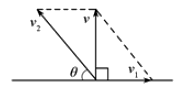
\includegraphics[width=0.3\linewidth]{image/kinamatics-1}\qquad\qquad 	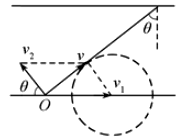
\includegraphics[width=0.2\linewidth]{image/kinamatics-2}
\end{center}

2. 想垂直到达河对岸,应该让船头与上游河岸保持一定的角度$ \theta $,船的运动如左图所示.
$ \cos\theta =v_1/v_2 =3/5 $,即船头与上游的夹角$\theta=\arccos⁡3/5$;船的合速度$ v=\sqrt{v_2^2-v_1^2}=4~\si{m/s} ,t=d/v=15~\si{s}  $.

3. 要使小船渡河时间最短,小船船头仍然应该垂直河岸渡河,渡河的最短时间$ t_{min} = d/v_2 = \SI{20}{s} $.
由于现在水流速度大于船在静水中的速度,船夫想要垂直到达河对岸的想法只能成为泡影,我们只能保证船的航程最短,但无法保证船垂直到达对岸.当船在静水中的速度$ v_2 $小于水流速度$ v_1 $时,合速度$ v $不可能与河岸垂直,只有当合速度$ v $方向越接近垂直河岸的方向,航程越短.
可由几何方法求得,以$ v_1 $的末端为圆心,以$ v_2 $的长度为半径作圆,从$ v_1 $的始端作此圆的切线,该切线方向即为最短航程的方向,如右图所示.
其中
\[
\cos\theta = v_2/v_1
 = 1/2,\qquad \theta =  60^\circ,\]
 由此可得最短航程
 \[
 s_{min} = \frac{d}{\cos\theta} = 120~\si{m}.
 \]


\end{app}



\begin{example}
	 有一条两岸平直、河水均匀流动、流速恒为$ v $的大河.小明驾着小船渡河,去程时船头指向始终与河岸垂直,回程时行驶路线与河岸垂直.去程与回程所用时间的比值为$ k $,船在静水中的速度大小相同,求小船在静水中的速度,结果用$ k $和$ v $表示。
	%	\begin{problemfig}
	%		\includegraphics[width=行宽比例\linewidth]{文件位置}
	%	\end{problemfig}
	
	\begin{taggedblock}{student}
		\vspace*{3cm}
	\end{taggedblock}
	
	%%%%%%%%答案
	\begin{taggedblock}{answer}
		【答案】:$ \frac{v}{\sqrt{1-k^2}} $
	\end{taggedblock}
	%%%%%%%%解析
	
	\begin{taggedblock}{analysis}
		【解析】:设船渡河时的速度为$ v_c $,
		当船头指向始终与河岸垂直,有$ t_1 =d/v_c $ ;
		当回程时行驶路线与河岸垂直,有$ t_2 =d/v_2 $ ;
		而回头时的船的合速度$ v_2 =\sqrt{v_c^2-v^2  }$;
		由于去程与回程所用时间的比值为$ k $,所以小船在静水中的速度大小为
	\[
	v_c = \sqrt{\frac{v^2}{1-k^2}} = \frac{v}{\sqrt{1-k^2}}.
	\]
		
	\end{taggedblock}
\end{example}



\begin{example}
	有一条两岸平直、河水均匀流动、流速恒为\SI{4}{m/s}的大河.初始时,船头与河岸成$ 37^\circ $,船刚好能垂直河岸运动.
	某时刻船的发动机出现障,船相对水的速度逐渐减小到零,船头方向不变.求此过程中,船相对地的速度的最小值.
	%	\begin{problemfig}
	%		\includegraphics[width=行宽比例\linewidth]{文件位置}
	%	\end{problemfig}
		\begin{taggedblock}{student}
		\vspace*{3cm}
	\end{taggedblock}

	%%%%%%%%答案
	\begin{taggedblock}{answer}
		答案:\SI{2.4}{m/s}
	\end{taggedblock}
	%%%%%%%%解析
	
	\begin{taggedblock}{analysis}
		解析:略
	\end{taggedblock}
\end{example}


\begin{example}
	玻璃板生产线上,宽\SI{9}{m}的成型玻璃板以$ 4\sqrt{3}~\si{m/s} $ 的速度连续不断地向前行进,在切割工序处,金刚钻的走刀速度为\SI{8}{m/s} ,为了使割下的玻璃板都成规定尺寸的矩形,金刚钻割刀的轨道应如何控制?切割一次的时间多长?
	%	\begin{problemfig}
	%		\includegraphics[width=行宽比例\linewidth]{文件位置}
	%	\end{problemfig}
	
	\begin{taggedblock}{student}
		\vspace*{3cm}
	\end{taggedblock}
	
	
	%%%%%%%%答案
	\begin{taggedblock}{answer}
		答案:\SI{2.25}{m/s}
	\end{taggedblock}

	%%%%%%%%解析
	\begin{taggedblock}{analysis}
		\marginpar{\centering 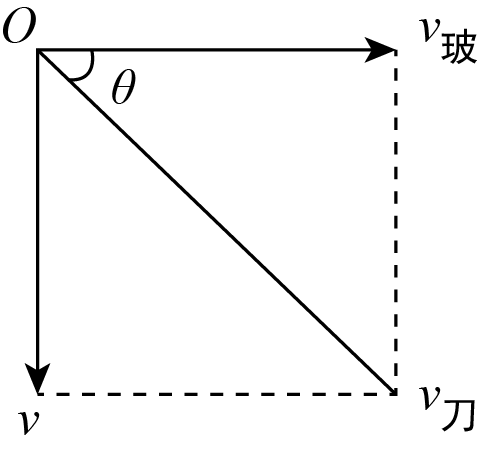
\includegraphics[width=\marginparwidth]{image/kinamatics-3.png}\figcaption{\theexample 题解析}  }
		解析: 要切成矩形,则割刀相对玻璃板的速度$ v $垂直玻璃板边缘,如图设$v_k$与$v_g$方向夹角为$ \theta $,$\cos\theta=v_g/v_k =(4√3)/8$,则$\theta=30^\circ$.
	这样$v = \sqrt{v_k^2-v_g^2} = \SI{4}{m/s}  $,时间$t=s/v=2.25\si{s} $.
	\end{taggedblock}
\end{example}


\begin{example}
	某汽车前方的挡风玻璃与水平方向成角度$\deg{37}$,当汽车以\SI{30}{m/s} 在水平地面上开行时,汽车司机看到雨滴垂直打在挡风玻璃上,实际虽然下雨但是没有风,计算雨滴下落的速度.
	%	\begin{problemfig}
	%		\includegraphics[width=行宽比例\linewidth]{文件位置}
	%	\end{problemfig}
	
	\begin{taggedblock}{student}
		\vspace*{2cm}
	\end{taggedblock}
	
	
	%%%%%%%%答案
	\begin{taggedblock}{answer}
		答案:\SI{40}{m/s}
	\end{taggedblock}
	%%%%%%%%解析
	\begin{taggedblock}{analysis}
		解析:略
	\end{taggedblock}
\end{example}


\begin{example}
	 一块板竖直地立在车上,车在雨中匀速行进一段给定的路程.木板板面与车前进方向垂直,其厚度可忽略.设空间单位体积中的雨点数目处处相等,雨点匀速竖直下落.下列诸因素中与落在木板上雨点的数目有关的因素是$ \underline{\qquad\qquad} $
	 
	 \begin{center}
	 	\small
	 		A.雨点下落的速度 \qquad  B.单位体积中的雨点数  \qquad C.车行进的速度  \qquad D.木板的面积
	 \end{center}

	
	%	\begin{problemfig}
	%		\includegraphics[width=行宽比例\linewidth]{文件位置}
	%	\end{problemfig}
	
	\begin{taggedblock}{student}
		\vspace*{1cm}
	\end{taggedblock}
	
	
	%%%%%%%%答案
	\begin{taggedblock}{answer}
		答案:BD
	\end{taggedblock}


	%%%%%%%%解析
	\begin{taggedblock}{analysis}
		解析:设单位体积中的雨滴数为$n_1$,汽车速度为$ v $,木板的面积为$S  $,在时间$ t $内,汽车行驶的距离$ x=vt $,落在木板面上雨点的数量n$ _2=n×V=n×vtS=nvtS $,单位时间内,落在木板面上雨点的数量$ n=n_1 vS $,由于距离一定落在木板上总雨点数$ n_{total}=n_1 tvS $.
	\end{taggedblock}
\end{example}



\begin{example}
	一个人以速度\SI{1}{m/s}向北漫步,感受到风从东边来,后来他的速度提高到\SI{2}{m/s},感受到风从东北方向吹来,求当他静止时,感受到风的方向和速度。
	%	\begin{problemfig}
	%		\includegraphics[width=行宽比例\linewidth]{文件位置}
	%	\end{problemfig}
	
	\begin{taggedblock}{student}
		\vspace*{3cm}
	\end{taggedblock}
	
	
	%%%%%%%%答案
	\begin{taggedblock}{answer}
		【答案】:东南风约\SI{14}{m/s}.
	\end{taggedblock}
	
	%%%%%%%%解析
	\begin{taggedblock}{analysis}
		【解析】:略
	\end{taggedblock}
\end{example}


\stitle{参考系变换}
在处理实际问题时,一般选择地面为参考系,但并不是所有问题都只能选择地面为参考系。如果能灵活巧妙地选择参考系,有时可以简化求解过程。

在处理运动学问题时,变换参考系时只需按照速度、位移、加速度变换公式进行相应变换即可。但是在处理动力学、能量问题时,可能涉及惯性力等复杂问题,要特别注意,这些内容我们会在后面模块中陆续介绍。

\begin{app}{擦肩而过}{}
	两个质点$A$、$B$同时从$P$、$Q$两点出发,分别以速度$\vec{v}_{1}$沿直线$AB$和以速度$\vec{v}_2$沿PR作匀速直线运动,$QR$和$QP$的夹角为$\alpha$,开始时$PQ$两点相距$l$,求此后两质点的最短距离。
	\begin{center}
		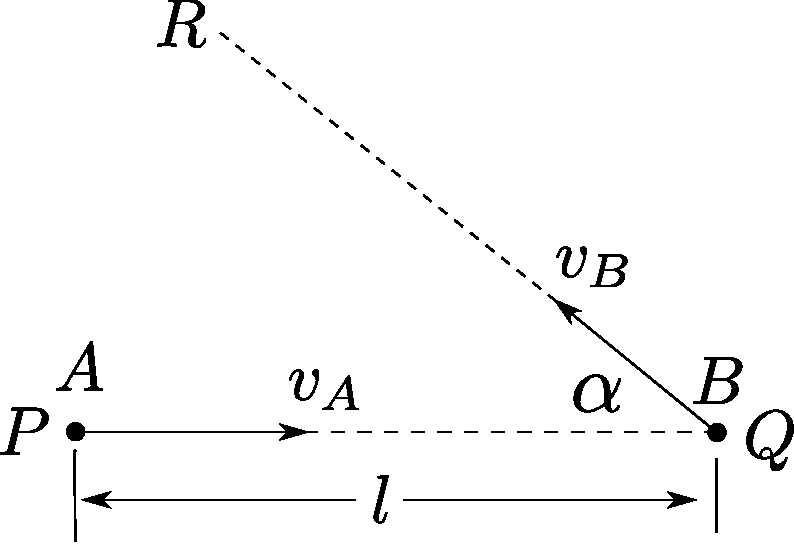
\includegraphics[width=0.3\linewidth]{image/motion-problem-29}
	\end{center}
	\tcblower
	\begin{center}
		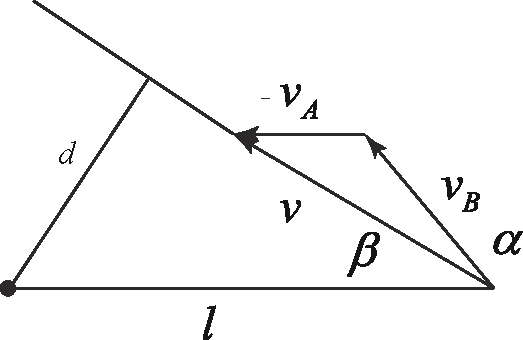
\includegraphics[width=0.3\linewidth]{image/motion-problem-1}
	\end{center}
	
	解:除了通常的解法以外还可以使用参考系变换的方法,若以A为参考系进行观察,B相对于A的速度满足
	\[
	\vec{v}_{B\rightarrow A} = 	\vec{v}_{B\rightarrow G}+	\vec{v}_{G\rightarrow A} = \vec{v_B}-\vec{v_A},
	\]
	上式中的$ G $代表与地面(ground)。
	如图所示给出了B相对于A速度的大小和方向,对于本题来说,最关键的是相对速度与相对连线方向的夹角$ \beta $,利用几何关系可得
	\[
	\sin\beta = \frac{v_B\sin\alpha}{\sqrt{v_A^2+v_B^2+2v_Av_B\cos\alpha}},
	\]
	其中分母为相对速度的大小,这里已经使用了余弦定律。
	利用前面得到的相对速度,不难求出在此后的运动过程中两者的最近距离
	\[
	d = l\sin\beta =\left( \frac{v_B\sin\alpha}{\sqrt{v_A^2+v_B^2+2v_Av_B\cos\alpha}}\right)l
	\]
	
\end{app}




\begin{example}
	. 一队步兵以$ v_1=1.5~\si{m/s}  $的速度匀速前进,队列长度为$ L=1200~\si{m} $ .通讯员从队尾到队首传达命令后,立即返回队尾,共用时间为$ t=10~\si{min} $ ,如果通讯员的速度大小始终保持不变,且传达命令和改变方向所用时间忽略不计,求通讯员的速度大小.
	%	\begin{problemfig}
	%		\includegraphics[width=行宽比例\linewidth]{文件位置}
	%	\end{problemfig}
	
	\begin{taggedblock}{student}
		\vspace*{3cm}
	\end{taggedblock}
	
	
	%%%%%%%%答案
	\begin{taggedblock}{answer}
		【答案】:$ v = 4.5~\si{m/s}. $
	\end{taggedblock}
	
	%%%%%%%%解析
	\begin{taggedblock}{analysis}
		【解析】:设通讯员的速度大小为$ v $,从队尾走到队首所用时间为$ t_1 $、再从队首走到队尾所用时间为$ t_2 $.
		
		方法一:选择地面参考系,
		通讯员由队尾走到队首的过程中,由位移关系有
		\[
		vt_1=v_1 t_1+L.
		\]
		通讯员由队首走回队尾的过程中,由位移关系有:
		\[
		vt_2+v_1 t_2=t.
		\]
		又因为$t_1+t_2=t$.		带入数据,联立可解得$v=4.5\si{m/s}$.
		
		方法二:选择一队步兵为参考系,以$ v_1 $方向为正方向:
		这时运动情景变为一队步兵静止不动,通讯员先以$ v-v_1 $的速度由队尾走到队首,再以$ -v-v_1 $的速度(即速度大小为$ v+v_1 $,方向与正方向相反)由队首走到队尾,所用的总时间为$ t=10\si{min} $.列出方程为:
		\[
		L/(v-v_1 )+L/(v+v_1 )=t.
		\]
		带入数据可解得:$v=4.5\si{m/s}$.
		
		其实不难发现,方法二的方程可以由方法一的方程组通过消元得到.在不同的参考系中都可
		以解决这个问题,但是方法二通过换参考系,使得思维难度下降,问题变简单了.
	
		
	\end{taggedblock}
\end{example}



\begin{example}
	有人逆水行舟,水速$ v_r=3\si{m/s}$ ,途中从船上掉下一漂浮物,10分钟后发现,并立即调头追赶,如果人划船速度大小保持$ v_s =5~\si{m/s}  $不变,则追上漂浮物需要多长时间.(注意:$ v_s =5~\si{m/s}  $是指船相对水的速度)
	%	\begin{problemfig}
	%		\includegraphics[width=行宽比例\linewidth]{文件位置}
	%	\end{problemfig}
	
	\begin{taggedblock}{student}
		\vspace*{3cm}
	\end{taggedblock}
	
	
	%%%%%%%%答案
	\begin{taggedblock}{answer}
		【答案】:10~\si{min}.
	\end{taggedblock}
	
	%%%%%%%%解析
	\begin{taggedblock}{analysis}
		【解析】:选择流动的河水为参考系.
		在此参考系中,漂浮物落水后不再运动,
		船以\SI{5}{m/s} 向前行驶10分钟后调头仍以同样的速度运动到漂浮物落水处,
		因船的往返速度和位移大小均相同,故往返时间必相同,即返回时间也为10分钟.
	
		
	\end{taggedblock}
\end{example}



\begin{example}
	 在宽为$ l $的河的两岸停着两艘小船,它们的连线与河岸成$ \alpha $角,已知两艘小船在静水中最大的划行速度分别为$ u_1,u_2 $,河水流速为$ v $.若它们同时出发,则各应向什么方向划行才能在最短时间内相遇,并求出此时间.
	%	\begin{problemfig}
	%		\includegraphics[width=行宽比例\linewidth]{文件位置}
	%	\end{problemfig}
	
	\begin{taggedblock}{student}
		\vspace*{3cm}
	\end{taggedblock}
	
	
	%%%%%%%%答案
	\begin{taggedblock}{answer}
		【答案】:见解析。
	\end{taggedblock}
	
	%%%%%%%%解析
	\begin{taggedblock}{analysis}
		【解析】: 两小船初始时相距$ l/\sin\alpha $ ,其方向与河岸成$ \alpha $角.
		设两船相对河岸的速度分别为$ \vec{v}_1,\vec{v}_2 $,则
		\[
		\vec{v}_1 = \vec{v}+\vec{u}_1,\qquad \vec{v}_2 = \vec{v}+\vec{u}_2,
		\]
		其中$ \vec{v} $为河水相对岸的速度。
		两船相对速度为
		\[
		\vec{v}_1 -\vec{v}_2 = 	\vec{u}_1 -\vec{u}_2,
		\]
		易知,当相对速度两船连线方向的投影最大时,则它们将用最短时间相遇.
		因此,要求$ \vec{u}_{1,2} $平行于两船连线方向,且相互接近($ \vec{u}_{1,2} $反向).所需时间为
		\[
		t = \frac{l }{(u_1+u_2)\sin\alpha}.
		\]
	.
	\end{taggedblock}
\end{example}



\begin{example}
	 如图所示,几辆相同的汽车以相等的速度v沿宽为c的平直公路行驶(不妨设向右行驶),每车宽为b,头尾间间距为a,则人能沿一条直线安全穿过马路时的最小速度是多少?
	 \marginpar{\centering 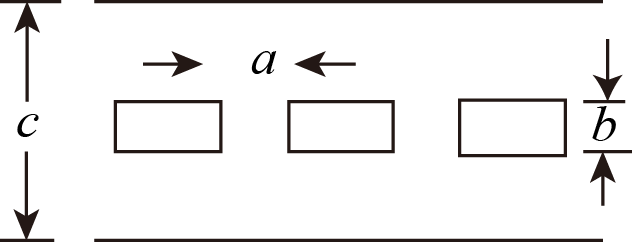
\includegraphics[width=\marginparwidth]{image/kinamatics-4.png}\figcaption{第\theexample 题} }
	%	\begin{problemfig}
	%		\includegraphics[width=行宽比例\linewidth]{文件位置}
	%	\end{problemfig}
	
	\begin{taggedblock}{student}
		\vspace*{2cm}
	\end{taggedblock}
	
	
	%%%%%%%%答案
	\begin{taggedblock}{answer}
		【答案】:$ v_{min} = \frac{b}{\sqrt{a^2+b^2}}v $
	\end{taggedblock}
	
	%%%%%%%%解析
	\begin{taggedblock}{analysis}
		
				\marginpar{\centering 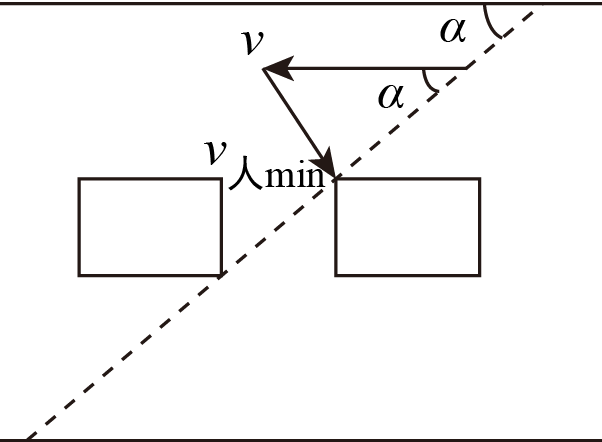
\includegraphics[width=\marginparwidth]{image/kinamatics-5.png}} 
		【解析】:这个情景也与小船过河问题有类似之处(人的运动方向可以变化,存在恒定速度运动的车流),不过分析起采要更复杂一些.
		本题在地面参考系中研究比较困难(主要是在地面参考系中不容易看出人相对车是如何运动的),因此我们选择车为参考系,
		如图所示,人刚好能正常穿过马路时(不与车辆相碰),应该相对车沿虚线方向运动,设虚线方向与水平方向夹角为$ \alpha $,则$ \sin\alpha=b/\sqrt{a^2+b^2} $,
		由于$v_{\text{人对车}}=v_{\text{人对地}}-v_{\text{车对地}}$,如图中几何关系所示,可知$v_{min}=v\sin\alpha=vb/\sqrt{a^2+b^2} $.
		当然本题中人相对车也可以沿其他直线路径过马路,但是这时路径与水平方向的夹角都大于图中a,对应的$ \vec{v} $都比图中的$ v_{min} $大,因此,图中情况所得的$ v_{min} $即为人安全穿过马路时的最小速度.

		
	\end{taggedblock}
\end{example}



\stitle{导数}
当我们研究一个函数自变量与因变量之间的关系时,除了它们数值上“静态的”对应关系外,往往还
需要有“运动”或“变化”的观点,即着眼于研究函数的变化趋势、增减快慢等,这也就是函数的“变化率”的
概念。



 当函数$  y=f(x) $的自变量 $ x $从$  x_0 $增加一个增量 $ \Delta x $,即从 $ x_0 $变为 $ x_0+\Delta x $,那么对应的函数值也从$  f(x_0) $变到 $ f(x_0+\Delta x) $,于是因变量 $ y $的增量:
 \[
 \Delta y =  f(x_0+\Delta x) -f(x_0),
 \]
 那么,$ \Delta y $和$ \Delta x $的增量比为
 \[
 \frac{\Delta y}{\Delta x} = \frac{f(x_0+\Delta x) -f(x_0)}{\Delta x},
 \]
 这个比值,就是函数在区间$  [x_0,x_0+\Delta x] $内的平均变化率。当 $ \Delta x\rightarrow 0 $时,上述 变化量比的极限就是函数在$ x_0 $处的变化率,数学上称其为$ y=f(x) $在$ x_0 $处对$ x $的导数 ,记作$  y' (x_0) $或者 $ f' (x_0) $,即
 \begin{equation}
  y' (x_0) = f' (x_0) = \lim_{ \Delta x\rightarrow 0}\frac{\Delta y}{\Delta x} =  \lim_{ \Delta x\rightarrow 0}\frac{f(x_0+\Delta x) -f(x_0)}{\Delta x} .
 \end{equation}
 除了$  y' (x_0) $、$  f' (x_0) $外,导数还常常写成微商的形式,如 $ dy/dx $、$  df/dx $、 $ \dv{x} f(x) $。
 这里需要指出的是, 函数$ f(x) $的导数$ f' (x) $本身也是关于$ x $的一个函数,不同的$ x $值对应的$ f' (x) $也不同 。
  \begin{figure}
\centering
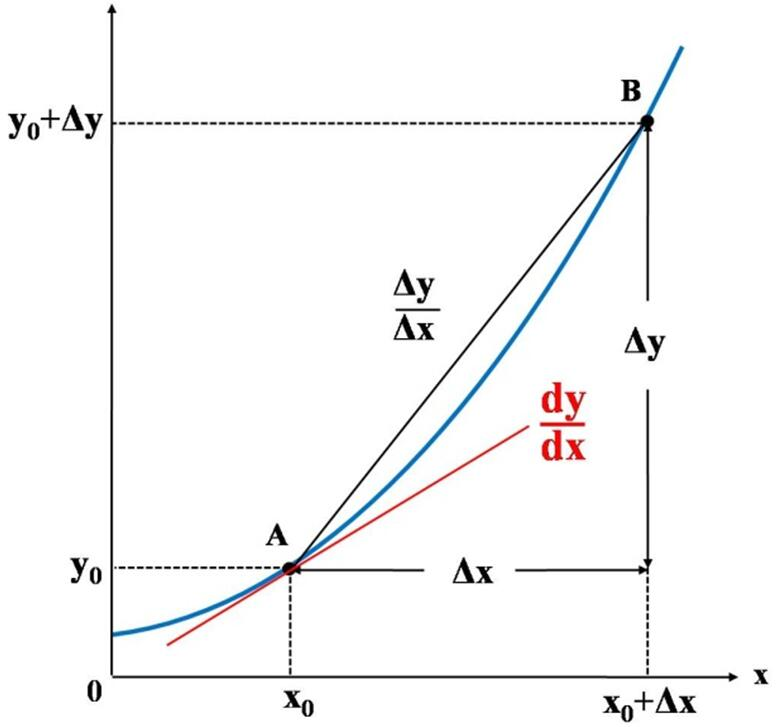
\includegraphics[width=0.5\linewidth]{image/kinamatics-6}
\caption{导数就是切线的斜率}
\label{fig:kinamatics-6}
\end{figure}


这里我们将从函数图像上来帮助大家理解导数“变化率”的概念。
如图\ref{fig:kinamatics-6}所示为某一函数的图像,我们在函数图像上任取一点 $ A(x_0,y_0) $,当自变量 $ x $有一增量$  \Delta x $时,函数值 $ y=f(x) $也会相应增加 $ \Delta y $,此时对应于函数图像上的另一点$  B(x_0+\Delta x,y_0+\Delta y) $,此时 $ \Delta y $与 $ \Delta x $的增量比即为直线 AB的斜率。当  $ \Delta x $逐渐减小时,  $ \Delta y $也会相应减小,此时 B点会沿着函数图像向 A点靠近。当  $ \Delta x \rightarrow 0 $时,直线 AB会变成函数图像在 A点的切线,即 $ y=f(x) $在 A点切线的斜率 $ k $就等于函数在 A点的导数,记作:
\begin{equation}
k = \dv{y}{x} = \lim_{ \Delta x\rightarrow 0}\frac{\Delta y}{\Delta x} =  \lim_{ \Delta x\rightarrow 0}\frac{f(x_0+\Delta x) -f(x_0)}{\Delta x}
\end{equation}
这里需要指出的是,直线的斜率 $ k $有正有负,那么一个函数的导数也有正有负。
当函数图像上某一点 $ A(x_0,y_0) $的切线斜率 $ k>0 $时,函数在此点的导数 $ f' (x_0)>0 $,说明函数值在 A点附近正在递增。
同理当函数图像上一点 $ A(x_0,y_0) $的切线斜率$ k<0 $时函数值会随着自变量的增加而减小。

\stitle{基本初等函数的导数}

 基本初等函数有常值函数、幂函数、指数函数、对数函数、三角函数、反三角函数 6种,基本函数的导数只能通过导数的定义(和反函数的性质)来求解,下面我们介绍高中阶段常见的前5种基本初等函数和它们的导数。
 
 
 \begin{description}
 	\item[常值函数]  常值函数 (也称常函数)是指函数值不发生改变(即是常数)的函数。常函数常以
 	\[
 	f(x) = \const \qquad or \qquad f(x) = C
 	\]
 表示。如$ f(x)=8.18 $。
 	由于常函数f(x)=C的值不随自变量x变化而变化,所以常函数的导数为$ f' (x)=0 $
 	
 	\item[幂函数] 以底数为自变量,幂为因变量,指数为常数的函数。幂函数常以$ f(x)=x^n $表示,这里的指数$ n $可以是任何有理数。
 	幂函数的导数$ f' (x)=nx^(n-1) $。
 	
 	\item[指数函数]以指数为自变量,幂为因变量,底数为常数的函数。指数函数以$ f(x)=a^x $表示,式中$ a>0 $且$ a\neq 1 $。
 	指数函数的导数$ f' (x)=a^x ln⁡a $。
 	特别地,当底数$ a $是自然常数$ e $(即$ a=e $)时,$ f' (x)=e^x $,即$ f(x)=e^x $的导数还是原函数本身。
 	\item[对数函数]以幂为自变量,指数为因变量,底数为常数的函数。对数函数以$f(x)=\log_a⁡x$表示,式中$ a>0 $且$ a\neq 1 $。
 	对数函数的导数$ f' (x)=1/(xln⁡a) $。
 	特别地,当底数$ a $是自然常数$ e $(即$ a=e $)时,$ f' (x)=1/x $。
 	\item[三角函数]以角度为自变量,角度对应任意两边的比值为因变量的函数。
 	在这里我们给出两个三角函数的导数,其余三角函数的导数可以通过后面我们介绍的求导法则来求解。正弦函数$ f(x)=\sin ⁡x $的导数$ f' (x)=\cos⁡ x $,余弦函数$ f(x)=\cos⁡ x $的导数$ f' (x)=-\sin ⁡x $。
 \end{description}

\stitle{函数求导法则}

 一般初等函数常常是由多个基本初等函数组合而成的,例如 $ y=\frac{1}{\sqrt{\sin x}}⁡ $)就是由 $ y=1/x $、 $ y=\sqrt{x} $、$  y=\sin⁡x $组合而成的。
 所以在求导运算中,需要定义一些求导的运算法则,它们可能通过导数的定义直接推导而得。
 
  设 $ f $和 $ g $都是可导函数, $ \alpha $和 $ \beta $都是常数,那么
  \begin{eqnarray}
  	(\alpha f+\beta g)' &=& \alpha f'+\beta g',\\
  	(fg)'&=&f'g+fg',\\
  	\left( \frac{f}{g} \right)'&=&\frac{f'g-fg'}{g^2}. 
  \end{eqnarray}


\begin{example}
	%%%%题干
	利用导数的性质求以下函数的导数
	\begin{eqnarray*}
	f(x)&=& x^2\cos x,\\
	f(x)&=& \tan x,\\
	f(x)&=&\frac{3x^2-2}{5x+1},\\
	f(x)&=& \frac{x\sin x+\cos x}{x\sin x-\cos x}.
				\end{eqnarray*}
	%%%%插图
	%	\begin{problemfig}
	%		\includegraphics[width=0.6\linewidth]{image/}
	%	\end{problemfig}
	
	\begin{taggedblock}{student}
		\vspace*{0cm}
	\end{taggedblock}
	
	
	%%%%答案
	\begin{taggedblock}{answer}
		答案:
	\end{taggedblock}
	
	
	%%%%解析
	\begin{taggedblock}{analysis}
		解析:
	\end{taggedblock}
\end{example}

如果函数 $ \varphi(x) $在 $ x_0 $处可导,函数$  f $在 $ u_0=\varphi(x_0) $处可导,则复合函数$  f(\varphi(x)) $在$  x_0 $处可导,且满足
\begin{equation}
f' (x)=f' (u_0)φ' (x_0),
\end{equation}
利用微分记号,复合函数求导可以简单表述如下
\begin{equation}
\dv{y}{x} = \dv{y}{u}\dv{u}{x}
\end{equation}

\begin{example}
	%%%%题干
	利用复合函数求导法则求以下函数的导数
	\begin{eqnarray*}
		f(x)&=&\cos(ax+b),\\
		f(x)&=&\sin^{10}x,\\
		f(x)&=&\sin(10 x),\\
		f(x)&=&\sqrt{x^2-1}.
	\end{eqnarray*}
	%%%%插图
	%	\begin{problemfig}
	%		\includegraphics[width=0.6\linewidth]{image/}
	%	\end{problemfig}
	
	\begin{taggedblock}{student}
		\vspace*{0cm}
	\end{taggedblock}
	
	
	%%%%答案
	\begin{taggedblock}{answer}
		答案:
	\end{taggedblock}
	
	
	%%%%解析
	\begin{taggedblock}{analysis}
		解析:
	\end{taggedblock}
\end{example}

\stitle{函数的极值}
 函数的导数刻画了函数的瞬时变化率,从而很好地描述了函数局部变化的性质。
 我们在导数的几何意义中已经提到了导数与函数单调性的关系。当一个函数在连续变化时,函数在 $ x=x_0 $处的导数满足 $ f' (x_0)>0 $,说明函数正在单调递增。
 同理,如果函数在 $ x=x_0 $处的导数满足$ f' (x_0)<0 $,说明函数正在单调递减。
 作为一个连续函数,随着$ x $的增加,往往会遇到函数值$ y=f(x) $有时递增有时递减,如图所示。当函数达到极大值或极小值时,显然有
 \begin{equation}
  f' (x_0)=0
 \end{equation}
所以我们往往可以通过导数等于零,来求解函数值达到极大或极小值时对应的$ x_0 $。


\begin{figure}
\centering
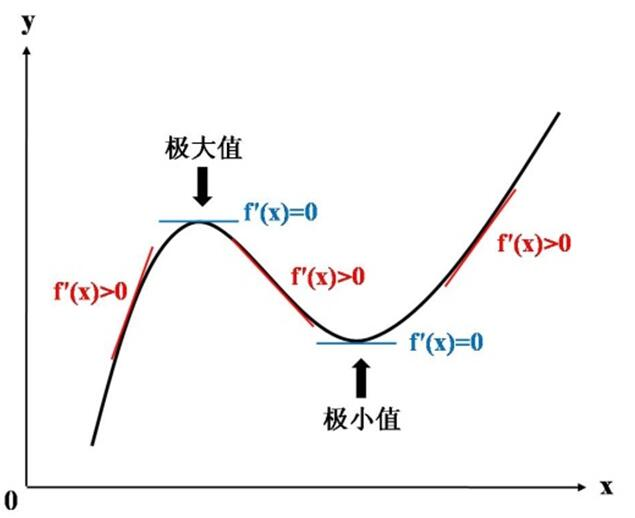
\includegraphics[width=0.5\linewidth]{image/kinamatics-7}
\caption{导数为零的点是函数的极值点}
\label{fig:kinamatics-7}
\end{figure}


\begin{example}
	%%%%题干
	 某商场销售某种商品的经验表明,该商品的每日销售量$  y $(单位为千克)与销售价格 $ x $(单位为元/千克)满足关系式
	 \[
	  y=a/(x-3)+10(x-6)^2,\qquad 3<x<6.
	 \]
	 求商品最理想的定价是多少。
  
	%%%%插图
	%	\begin{problemfig}
	%		\includegraphics[width=0.6\linewidth]{image/}
	%	\end{problemfig}
	
	\begin{taggedblock}{student}
		\vspace*{2cm}
	\end{taggedblock}
	
	
	%%%%答案
	\begin{taggedblock}{answer}
		答案:
	\end{taggedblock}
	
	
	%%%%解析
	\begin{taggedblock}{analysis}
		解析:
	\end{taggedblock}
\end{example}

\begin{example}
	%%%%题干
	某单位用木料做如图所示的框架,框架的下部是边长分别为$ x $、$ y $(单位为米)的矩形,上面是等腰直角三角形.要求框架的总面积为\SI{8}{m^2},问$ x $、$ y $分别为多少时用料最省?
	%%%%插图
		\begin{flushright}
			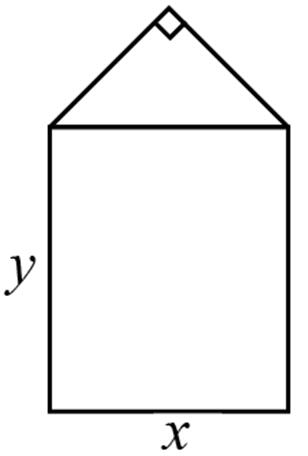
\includegraphics[width=0.2\linewidth]{image/kinamatics-8.png}
		\end{flushright}
	
	\begin{taggedblock}{student}
		\vspace*{0cm}
	\end{taggedblock}
	
	
	%%%%答案
	\begin{taggedblock}{answer}
		答案:
	\end{taggedblock}
	
	
	%%%%解析
	\begin{taggedblock}{analysis}
		解析:
	\end{taggedblock}
\end{example}
% !TEX root = ../zz-lecture.tex


\chapter{牛顿定律}

 牛顿运动定律是高中物理的基础,贯穿于高中物理的各个部分。
 在高中物理课程中,我们学习了牛顿运动定律的具体内容和基本应用。
 在未来的两次课中,我们将进一步研究牛顿第二定律(涉及分解加速度、加速度关联等问题)以及在非惯性系中如何使用牛顿第二定律。
 
 \stitle{牛顿第二定律}
 
 
 牛顿第二定律是矢量定律,因此可以分方向使用:
 \begin{equation}
 F_i = ma_i,
 \end{equation}
 其中$ i=1,2,3 $可以理解为力和加速度在给定直角坐标系中的$ x,y,z $分量。
在常规的高考问题中,一般是将外力沿加速度方向和垂直加速度方向进行正交分解,列出分量方程。
在一些复杂问题中,分解加速度列出分量方程可能会使问题更简化。


% !TEX root = ../zz-lecture.tex


\chapter{非惯性参考系}
我们首先回忆一下学习牛顿运动定律时涉及的一些概念。牛顿第一定律成立的参考系称为惯性参考系;例如地面以及相对地面静止或匀速直线运动的参考系都是惯性系;牛顿第二定律只在惯性系中成立,在非惯性系中不成立,例如下面这个情景:
静止的火车车厢内有一水平的光滑桌面,桌面上有一个静止的小球;现在使火车突然(相对地面)向左加速,加速度为$ a_s $(规定向左为正方向),这时小球将如何运动呢?

\marginpar{\centering 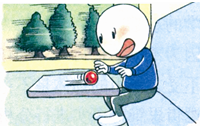
\includegraphics[width=\marginparwidth]{image/NIR-1}\figcaption{突然加速的火车} \label{fig:}}

地面上的观察者发现小球将静止在原地,这是符合牛顿运动定律的;而以车厢为参考系观察会发现小球以$-a_s$相对于车厢做加速运动,小球没有受到水平方向的作用力却产生了加速度,这显然是不符合牛顿运动定律的(实际是牛顿运动定律在这个参考系中不适用)。

\stitle{惯性力}

假设车厢中的人熟知牛顿运动定律,尤其对加速度一定是由力引起的印象至深,以致在任何场合下,他都强烈地要求保留这一认知。
于是车上的人说:小球之所以对小车有加速度$ -a_s $,是因为受到了一个指向右方的作用力,且力的大小为$ ma_s $;物理上把人为引入的$ -ma_s $这个力命名为惯性力。
需要注意的是: 惯性力是一种假想的力,不是物体间的真实相互作用,因此没有施力物体,也没有反作用力。
由于在非惯性系中研究动力学问题有一定难度,因此我们首先研究平动非惯性系的简单情况,对于转动参考系等复杂情况在后面展开。




假设质量为$ m $的物体相对地面的加速度为$ \vec{a} $,所受的合外力为$ \vec{F} $,某参考系S相对地面做平动,加速度为$\vec{a}_s $(即参考系S为非惯性系)。
在地面参考系中,根据牛顿第二定律可得
\[
\vec{F} = m\vec{a}.
\]
根据相对运动的定义,物体$ m $相对参考系S的加速度
\begin{equation}
\vec{a'} = \vec{a}-\vec{a}_s,
\end{equation}
两式联立可得:
\begin{equation}
\vec{F} = m\vec{a}'+m\vec{a}_s,
\end{equation}
将上式稍加变形得到
\begin{equation}
\vec{F}-m\vec{a}_s = m\vec{a}'.
\end{equation}
如果把上式左边$-m \vec{a}_s$看成一个力,(即前面所说的惯性力),我们可以把上式理解成非惯性系中的牛顿第二定律,即在非惯性系中,惯性力与物体所受真实力的合力共同产生物体相对该参考系的加速度。

为了在非惯性系中仍然可以使用牛顿第二定律解决动力学问题,需要对牛顿第二定律做些修正。
在非惯性系中,惯性力与物体所受真实力的合力提供物体的加速度,即
\begin{equation}
\vec{F}+\vec{f}_i = m\vec{a}',
\end{equation}
对于平动非惯性系$ \vec{f}_i = -m\vec{a}_s $(其中$ \vec{a}_s $是非惯性系相对地面的加速度),惯性力的作用点作用在质心上。
需要注意的是对于转动非惯性系,惯性力会比较复杂,可能不止一项。


\begin{example}
	%%%%题干
	若不考虑太阳和其他星体的作用,则地球——月球系统可以看成孤立系统.把地球和月球都看作是质量均匀分布的球体,它们的质量分别为$ M $、$ m $,月心和地心间的距离为$ R $,万有引力常量为$ G $.学生甲以地心为参考系,利用牛顿第二定律和万有引力定律得到月球相对于地心参考系的加速度为$a_m=GM/R^2$ ;学生乙以月心为参考系,同样利用牛顿第二定律和万有引力定律,得到地球相对于月心参考系的加速度为$a_e=Gm/R^2$ .两位同学求出的地月之间的相对加速度大小是不同的,这是不合理的,请定性解释原因.
	%%%%插图
	%	\begin{problemfig}
	%		\includegraphics[width=0.6\linewidth]{image/}
	%	\end{problemfig}
	
	\begin{taggedblock}{student}
		\vspace*{2cm}
	\end{taggedblock}
	
	
	%%%%答案
	\begin{taggedblock}{answer}
		答案:不对。
	\end{taggedblock}
	
	
	%%%%解析
	\begin{taggedblock}{analysis}
		解析:因为地球受到月球的引力作用、月球受到地球的引力作用.它们相对于惯性参考系都有加速度,因此它们都不是惯性参考系.在非惯性系中应用牛顿第二定律时,必须引入惯性力,两位同学都没有引入惯性力,因此算出的结果都是不对的.
	\end{taggedblock}
\end{example}


\begin{example}
	%%%%题干
	 如图所示,被水平拉伸的轻弹簧右端拴在小车壁上,左端拴一质量为\SI{10}{kg} 的物块M.小车静止不动,弹簧对物块的弹力大小为\SI{5}{N}时,物块处于静止状态.当小车向右做加速运动,且加速度逐渐由0增加到\SI{1}{m/s^2}的过程中
	 
	 A. 物块M相对小车仍静止; 
	 
	 B. 物块M受到的摩擦力一直减少; 
	 
	 C. 物体M受到的摩擦力一直增大; 
	 
	 D. 物体M受到的摩擦力先减少后增大.
	 
	 \marginpar{\centering 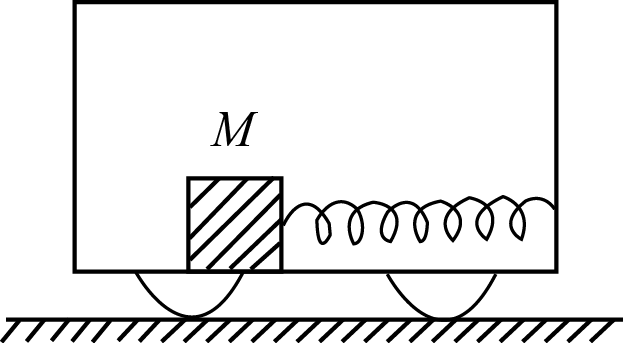
\includegraphics[width=\marginparwidth]{image/NIR-2.png}\figcaption{第\theexample 题} \label{fig:}}
	%%%%插图
	%	\begin{problemfig}
	%		\includegraphics[width=0.6\linewidth]{image/}
	%	\end{problemfig}
	
	\begin{taggedblock}{student}
		\vspace*{2cm}
	\end{taggedblock}
	
	
	%%%%答案
	\begin{taggedblock}{answer}
		答案:AD
	\end{taggedblock}
	
	
	%%%%解析
	\begin{taggedblock}{analysis}
		解析: 引入惯性力的概念,此时相当于给物体增加了一个水平向左的惯性力,而且此力的大小从0开始逐渐增大到\SI{10}{N} ,按照题中条件,摩擦力可以达到\SI{5}{N},因此物体始终与小车相对静止.摩擦力先减小再反向增大.
	\end{taggedblock}
\end{example}



\begin{example}
	%%%%题干
	如图,水平地面上有一楔形物体b,b的斜面上有一小物块a;a与b之间、b与地面之间均存在摩擦.已知楔形物体b静止时,a静止在b的斜面上.现给a和b一个共同的向左的初速度,与a和b都静止时相比,此时可能
	
	A.a与b之间的压力减少,且a相对b向下滑动
	
	B.a与b之间的压力增大,且a相对b向上滑动
	
	C.a与b之间的压力增大,且a相对b静止不动
	
	D.  b与地面之间的压力不变,且a相对b向上滑动
	
	\marginpar{\centering 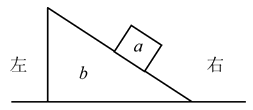
\includegraphics[width=\marginparwidth]{image/NIR-3}\figcaption{第\theexample 题} \label{fig:}}
	%%%%插图
	%	\begin{problemfig}
	%		\includegraphics[width=0.6\linewidth]{image/}
	%	\end{problemfig}
	
	\begin{taggedblock}{student}
		\vspace*{2cm}
	\end{taggedblock}
	
	
	%%%%答案
	\begin{taggedblock}{answer}
		答案:BC
	\end{taggedblock}
	
	
	%%%%解析
	\begin{taggedblock}{analysis}
		解析:本题同样可以在地面参考系中分析,但由于存在多种可能性,讨论起来比较复杂.下面我们以b为参考系,借助惯性力来分析.
		\marginpar{\centering 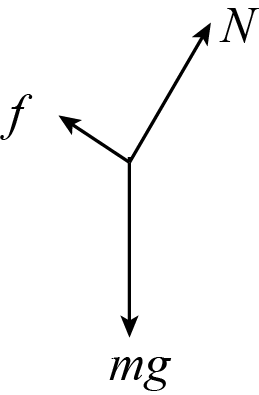
\includegraphics[width=0.6\marginparwidth]{image/NIR-4.png} }
		首先,a、b均静止时,在地面参考系中可知a受到重力$ mg $、支持力$ N $、摩擦力$ f $保持平衡,如图所示.
		当a、b向左运动时,由于地面存在摩擦力,因此b应有向右的加速度,做减速运动,以b为参考系,物块a的受力应增加一个水平向左的惯性力.在此参考系中,物块a在垂直斜面方向没有加速度,由平衡条件可知,支持力$ N $一定增大.在沿斜面方向分析可知:摩擦力可以减小或反向增大,因此,物块a可能继续保持静止或沿斜面向上滑动,但绝不可能沿斜面向下滑动(因为原来的静摩擦力小于最大静摩擦力),BC正确.
		
	\end{taggedblock}
\end{example}


\begin{example}
	%%%%题干
	如图所示,汽车内固定有一个倾角为$ \deg{37} $的斜面,斜面表面光滑,底部有一个质量为$ m $的小物块,开始时系统静止,某时刻汽车突然开始向左以加速度$ a $做匀加速运动.要使物体沿斜面向上运动,则$ a $至少多大.
	\marginpar{\centering 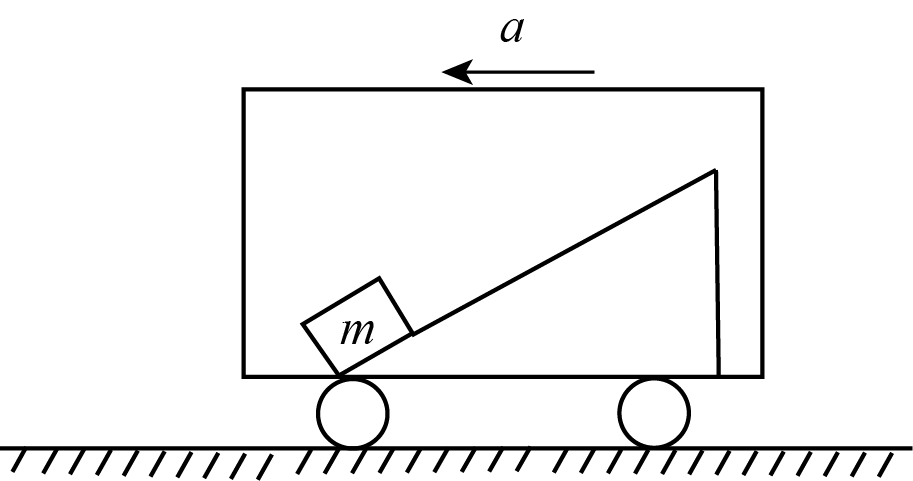
\includegraphics[width=\marginparwidth]{image/NIR-5.png}\figcaption{第\theexample 题} \label{fig:}}
	%%%%插图
	%	\begin{problemfig}
	%		\includegraphics[width=0.6\linewidth]{image/}
	%	\end{problemfig}
	
	\begin{taggedblock}{student}
		\vspace*{2cm}
	\end{taggedblock}
	
	
	%%%%答案
	\begin{taggedblock}{answer}
		答案:$ a>\frac{3}{4}g $
	\end{taggedblock}
	
	
	%%%%解析
	\begin{taggedblock}{analysis}
		解析:以斜面为参考系,物块受到水平向右的力$ F=ma $作用,要使物块沿斜面向上运动,则沿斜面方向$ F\cos\theta-mg\sin\theta>0 $,解得$a>3/4 g$.
	\end{taggedblock}
\end{example}


\begin{example}
	%%%%题干
	 质量为 $ M $的楔子置于光滑水平面上,给楔子施加水平推力 $ F $,要使质量为 $ m $的小球沿其倾角 $ \alpha $的粗糙斜面向上滚动,求$ F $的最小值。
	%%%%插图
	%	\begin{problemfig}
	%		\includegraphics[width=0.6\linewidth]{image/}
	%	\end{problemfig}
	
	\begin{taggedblock}{student}
		\vspace*{1cm}
	\end{taggedblock}
	
	
	%%%%答案
	\begin{taggedblock}{answer}
		答案:$ (M+m)g\tan\alpha $
	\end{taggedblock}
	
	
	%%%%解析
	\begin{taggedblock}{analysis}
		解析:当球刚好要沿斜面向上滚动时 $ F $有最小值,此时,对整体有: $ F=(M+m)a $.
		在斜面参考系中,球刚好能滚动,因此以球和斜面接触点为轴,小球所受力矩平衡,有: 
		\[
		mar\cos\alpha = mgr\sin\alpha,
		\]
	联立解得: $F=(M+m)g\tan\alpha⁡$.
		
	\end{taggedblock}
\end{example}


\begin{example}
	%%%%题干
	 一辆汽车质量为$ m $,前后轮相距$ 2l $,质心在车辆中心、距地面高度为$ h $.初始时车辆在平直路面做匀速直线运动,突然遇到紧急情况急刹车停下,为保证车辆不向前翻倒,则刹车过车中加速度最大为多少(地面摩擦因数足够大,不考虑车辆滑动)
	 \marginpar{\centering 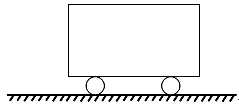
\includegraphics[width=0.8\marginparwidth]{image/NIR-6.png}\figcaption{第\theexample 题} }
	%%%%插图
	%	\begin{problemfig}
	%		\includegraphics[width=0.6\linewidth]{image/}
	%	\end{problemfig}
	
	\begin{taggedblock}{student}
		\vspace*{2cm}
	\end{taggedblock}
	
	
	%%%%答案
	\begin{taggedblock}{answer}
		答案:$\frac{gl}{h}$
	\end{taggedblock}
	
	
	%%%%解析
	\begin{taggedblock}{analysis}
		解析:略
	\end{taggedblock}
\end{example}



\begin{example}
	%%%%题干
	 如图所示,在以一定加速度$ a $行驶的车厢内,有一长为$ l $,质量为$ m $的棒AB靠在光滑的后壁上,棒与车箱底之间的动摩擦因数为$ \mu $.为了使棒不滑动,棒与竖直平面所成的夹角$ \theta $应在什么范围内?
	 \marginpar{\centering 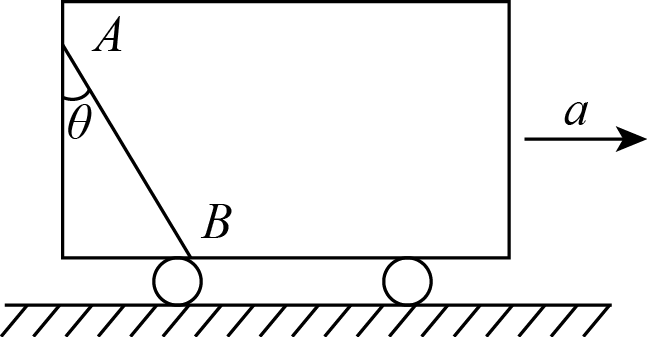
\includegraphics[width=\marginparwidth]{image/NIR-7.png}\figcaption{第\theexample 题} \label{fig:}}
	%%%%插图
	%	\begin{problemfig}
	%		\includegraphics[width=0.6\linewidth]{image/}
	%	\end{problemfig}
	
	\begin{taggedblock}{student}
		\vspace*{2cm}
	\end{taggedblock}
	
	
	%%%%答案
	\begin{taggedblock}{answer}
		答案:$ \arctan\frac{a-2\mu g}{g}\le \theta \le \arctan\frac{a+2\mu g}{g} $
	\end{taggedblock}
	
	
	%%%%解析
	\begin{taggedblock}{analysis}
		\marginpar{\centering 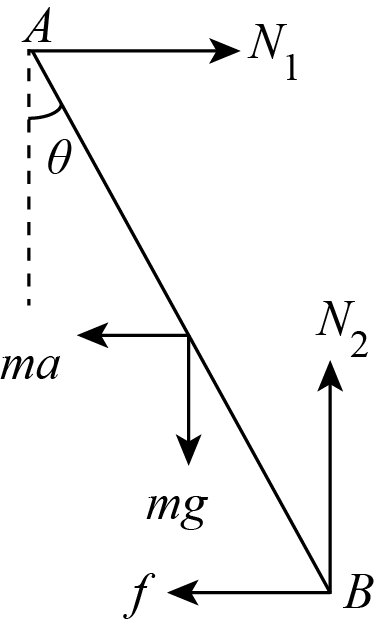
\includegraphics[width=0.6\marginparwidth]{image/NIR-8}}
		解析:以车厢为参照系,惯性力的作用点在棒的重心处,
		当$ \theta $取最大值时,棒AB刚好不滑动,受力如图所示,此时B端所受摩擦力的方向水平向左,且达最大静摩擦力,
		以A点为轴,由力矩平衡条件得
		\[
		ma\frac{l}{2}\cos\theta+fl\cos\theta+mg\frac{l}{2}\sin\theta = N_2l\sin\theta,
		\]
		又由受力平衡条件得:$N_2=mg$,$		f=\mu N_2$,解得
		\[
		\theta_{max} = \arctan\frac{a+2\mu g}{g}.
		\]
		同理,当$ \theta $取最小值时,棒的B端所受摩擦力方向水平向右,
		由力矩平衡条件得:
		\[
			ma\frac{l}{2}\cos\theta+mg\frac{l}{2}\sin\theta = N_2l\sin\theta+fl\cos\theta,
		\]
	可解得$ θ_{min}=arctan⁡(a-2μg)/g $,综上所述,要使棒不滑动,应满足$ \arctan\frac{a-2\mu g}{g}\le \theta \le \arctan\frac{a+2\mu g}{g} $。
		
		
	\end{taggedblock}
\end{example}


\begin{example}
	%%%%题干
	如图所示,质量为$ m $的物体放置在倾角为$ \alpha $的斜面上,且用绳连接在墙上,不计一切摩擦,当斜面以加速度$ a $向右运动时,求绳上的拉力.
	\marginpar{\centering 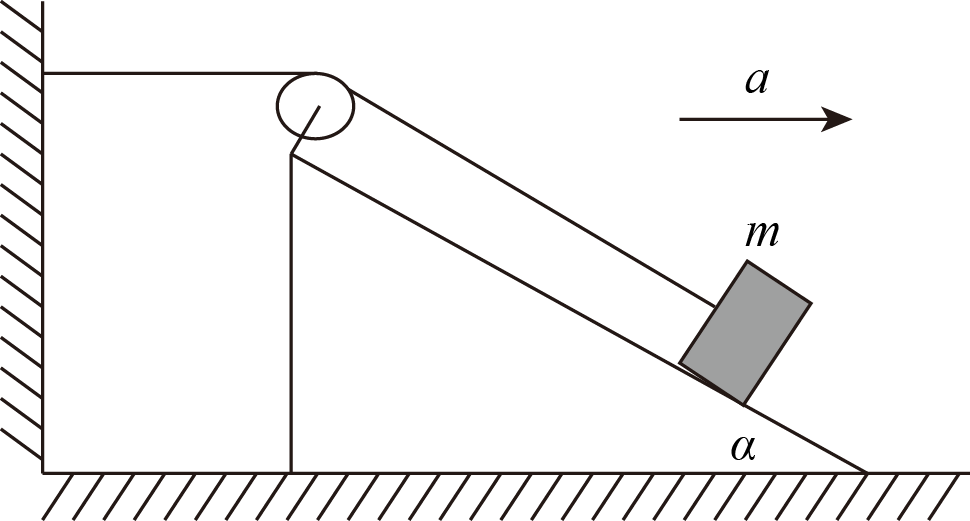
\includegraphics[width=\marginparwidth]{image/NIR-9.png}\figcaption{第\theexample 题} \label{fig:}}
	%%%%插图
	%	\begin{problemfig}
	%		\includegraphics[width=0.6\linewidth]{image/}
	%	\end{problemfig}
	
	\begin{taggedblock}{student}
		\vspace*{2cm}
	\end{taggedblock}
	
	
	%%%%答案
	\begin{taggedblock}{answer}
		答案:$ ma-ma\cos\alpha+mg\sin\alpha $
	\end{taggedblock}
	
	
	%%%%解析
	\begin{taggedblock}{analysis}
			\marginpar{\centering 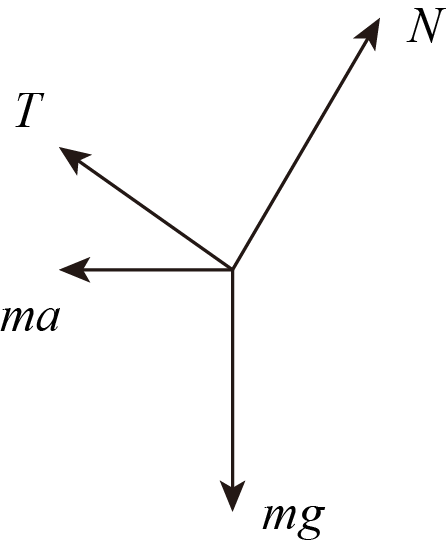
\includegraphics[width=0.6\marginparwidth]{image/NIR-10}}
		解析:本题在地面参考系中研究,$ m $的运动比较复杂,求解有一定难度,因此我们以斜面为参考系考虑这个问题;
		以斜面为参考系,物体受到重力$ mg $、支持力$ N $、拉力$ T $、惯性力$ ma $,如图所示,墙相对斜面以加速度$ a $拉绳子,所以物体沿斜面方向的加速度大小也是$ a $;
		沿斜面方向应用牛顿第二定律得:
		\[
		T+ma\cos\alpha-mg\sin\alpha=ma
		\]
		解得:$ T=ma-ma\cos\alpha+mg\sin\alpha $⁡α.
	
		
	\end{taggedblock}
\end{example}


\begin{example}
	%%%%题干
	 如图所示,与水平面成$ \theta $角的光滑棒AB上有一滑套C,开始时与棒的A端相距为$ l $,相对棒静止.当棒保持倾角$ \theta $不变沿水平面匀加速运动,加速度为$a(a>g\tan\theta)$时,求滑套C从棒的A端滑出所经历的时间.
	 	\marginpar{\centering 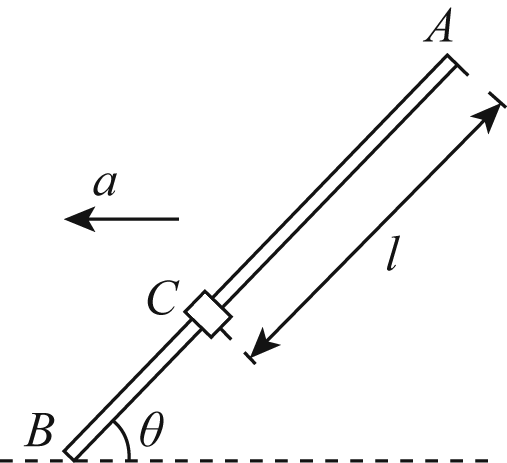
\includegraphics[width=\marginparwidth]{image/NIR-11.png}\figcaption{第\theexample 题} \label{fig:}}
	%%%%插图
	%	\begin{problemfig}
	%		\includegraphics[width=0.6\linewidth]{image/}
	%	\end{problemfig}
	
	\begin{taggedblock}{student}
		\vspace*{2cm}
	\end{taggedblock}
	
	
	%%%%答案
	\begin{taggedblock}{answer}
		答案:$ \sqrt{\frac{2l}{a\cos\theta-g\sin\theta}} $.
	\end{taggedblock}
	
	
	%%%%解析
	\begin{taggedblock}{analysis}
		\marginpar{\centering 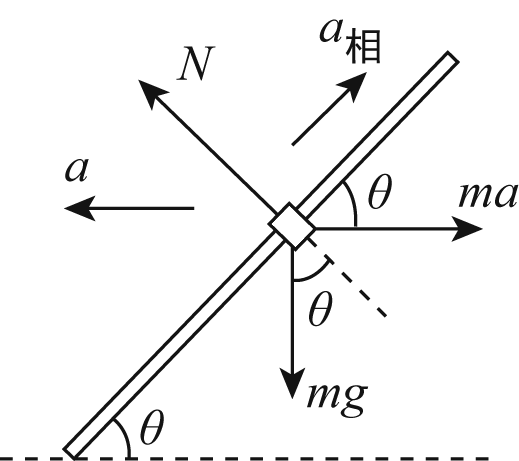
\includegraphics[width=0.8\marginparwidth]{image/NIR-12.png}}
		解析:以棒为参照系,对滑套C受力分析如图所示,
			由牛顿第二定律有
			\[
			ma\cos\theta-mg\sin\theta = ma_r,
			\]
		滑套相对杆做匀加速直线运动,由运动学公式
		\[
		l = \frac{1}{2}a_rt^2,
		\]
		联立解得
		\[
		t = \sqrt{\frac{2l}{a\cos\theta-g\sin\theta}} 
		\]
		
	\end{taggedblock}
\end{example}



\begin{example}
	%%%%题干
	在光滑的水平面上有一质量为$ M $、倾角为$ \theta $的光滑斜面,其上有一质量为$ m $的物块,如图所示.求物块在下滑的过程中对斜面压力的大小。
		 	\marginpar{\centering 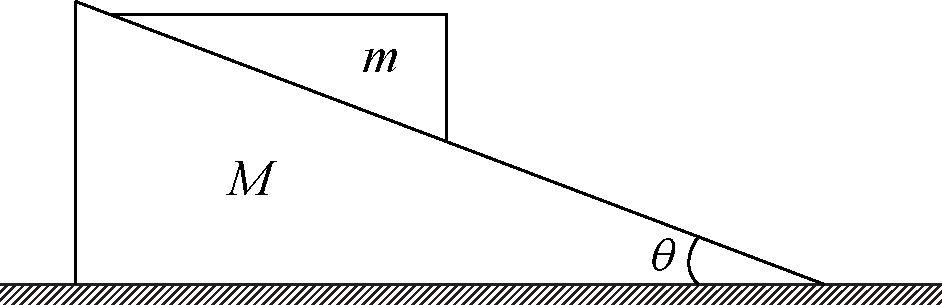
\includegraphics[width=\marginparwidth]{image/NIR-13.png}\figcaption{第\theexample 题} \label{fig:}}
	%%%%插图
	%	\begin{problemfig}
	%		\includegraphics[width=0.6\linewidth]{image/}
	%	\end{problemfig}
	
	\begin{taggedblock}{student}
		\vspace*{2cm}
	\end{taggedblock}
	
	
	%%%%答案
	\begin{taggedblock}{answer}
		答案:
	\end{taggedblock}
	
	
	%%%%解析
	\begin{taggedblock}{analysis}
		\begin{center}
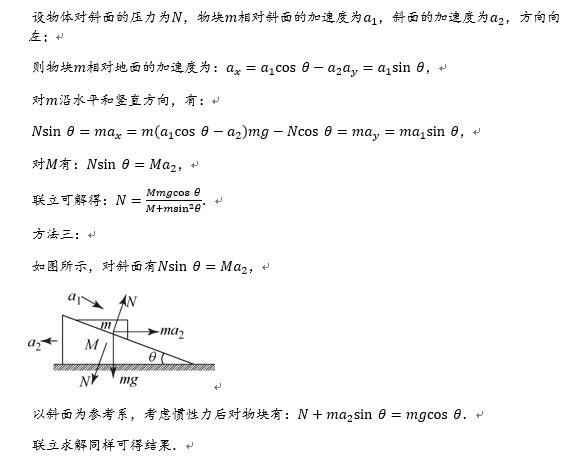
\includegraphics[width=0.9\linewidth]{image/NIR-14}
\end{center}

		
	\end{taggedblock}
\end{example}

\begin{example}
	%%%%题干
	如图所示,光滑的直角三角形斜楔C,质量不计,放置在光滑水平地面上,两侧各自放一个质量为$ m $的物块A、B,静止释放,计算释放后C的加速度.
			 	\marginpar{\centering 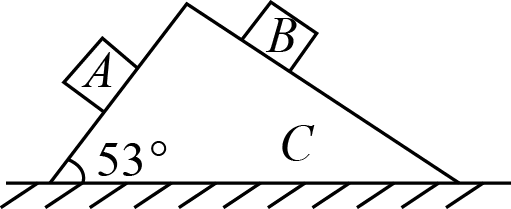
\includegraphics[width=\marginparwidth]{image/NIR-15.png}\figcaption{第\theexample 题} \label{fig:}}
	%%%%插图
	%	\begin{problemfig}
	%		\includegraphics[width=0.6\linewidth]{image/}
	%	\end{problemfig}
	
	\begin{taggedblock}{student}
		\vspace*{2cm}
	\end{taggedblock}
	
	
	%%%%答案
	\begin{taggedblock}{answer}
		答案:$ a=0 $
	\end{taggedblock}
	
	
	%%%%解析
	\begin{taggedblock}{analysis}
				\begin{center}
					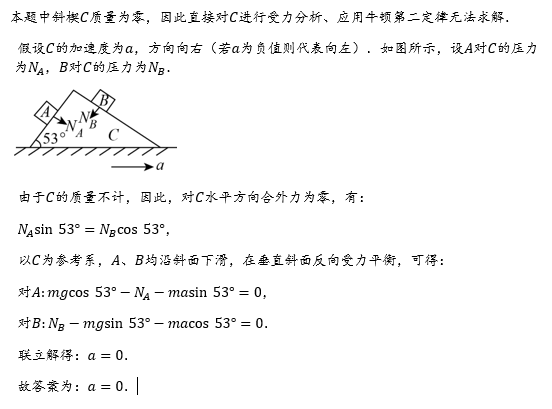
\includegraphics[width=0.9\linewidth]{image/NIR-16}
				\end{center}
	\end{taggedblock}
\end{example}
% !TEX root = ../zz-lecture.tex


\chapter{动量及其守恒}
动量和能量是高考的重点,也是高中物理课程的重点,同学们平时已经进行了大量的练习。
在本章中,我们对动量的内容进行一些拓展,主要包括二维情况、流体问题及质心系的应用。

\stitle{动量定理}

 在高中课程中我们已经学习过动量定理,并指出动量定理是矢量式,但所研究的问题基本都是一维情况。
 在这个模块中,我们研究一些二维平面问题。
 在应用动量定理时,既可以在某一方向使用,也可以通过正交分解在两个方向上同时使用,即
 \begin{equation}
 	I_i = \Delta p_i,\qquad i=1,2,3
 \end{equation}
 这里的角标$ i $可以理解为矢量在给定直角坐标系中的三个分量值。
 具体方法请大家结合例题学习。
 
 
 \begin{app}{粗糙表面的反弹}{}
 	某小球质量为$ m $,与地面之间的动摩擦系数为$ \mu $,现将小球从高度为$ h $处以初速度$ v_0 $平抛.小球与地面碰撞后,竖直方向的分速度大不变,求小球与地面碰撞后水平方向的分速度大小(假设$ v_0 $很大,小球与地面碰撞后水平方向的分速度不会减为零,且碰撞过程时间极短,重力冲量不计).
 	\tcblower
 	
 	以竖直向上为$ y $轴正方向,初速度$ v_0 $方向为$ x $轴正方向.
 	 	小球落地时竖直方向速度$ v_y = -\sqrt{2gh} $,
 	小球与地面碰撞过程,根据碰撞前后的运动状态变化,对水平、竖直方向分别应用动量定理得:
 	\[
 	I_y=(mv_y)-(-mv_y),\qquad I_x = \mu I_y = mv_x'-mv_0.
 	\]
 	这里已经使用了摩擦力时刻正比于正压力的事实,将以上两式联立不难得到弹起的水平速率
 	\[
 	v_x' = v_0-2\mu\sqrt{2gh}.
 	\]
 
 	
 \end{app}
 
 \begin{example}
 	%%%%题干
 	一袋面粉(可看做质点)沿着与水平面成$ \alpha = \deg{60} $角的光滑斜面,从高$ H $处无初速地滑下,落到水平地板上(不弹起),碰撞过程时间极短,不计重力冲量,袋与地板之间的动摩擦因数$ \mu = 0.7 $,问袋停在何处?
 	%%%%插图
 	%	\begin{problemfig}
 	%		\includegraphics[width=0.6\linewidth]{image/}
 	%	\end{problemfig}
 	
 	\begin{taggedblock}{student}
 		\vspace*{2cm}
 	\end{taggedblock}
 	
 	
 	%%%%答案
 	\begin{taggedblock}{answer}
 		答案:0.5~\si{m}.
 	\end{taggedblock}
 	
 	
 	%%%%解析
 	\begin{taggedblock}{analysis}
 	\begin{center}
\includegraphics[width=0.8\linewidth]{image/NIR-17}
\end{center}

 	\end{taggedblock}
 \end{example}
 
 \begin{example}
 	%%%%题干
 	 质量足够大的长平板从$ t=0 $时刻开始在水平方向上由静止出发朝右匀加速运动,加速度大小为$ a $.如图所示,在板的上方$ H $高处有一静止的小球,在$ t=0 $时刻自由下落,而后与平板发生碰撞.设小球与平板接触时的滑动摩擦系数$ \mu=0.1 $,小球反弹高度也为$ H $.将小球反弹离开平板时相对地面参考系的速度方向与朝右的水平方向夹角记为$ \beta $,试求$ \tan\beta $与$ a $的关系.(碰撞过程时间极短,重力冲量不计)
 	 
 	 \marginpar{\centering \includegraphics[width=\marginparwidth]{image/momentum-1.png}\figcaption{第\theexample 题 } \label{fig:}}
 	%%%%插图
 	%	\begin{problemfig}
 	%		\includegraphics[width=0.6\linewidth]{image/}
 	%	\end{problemfig}
 	
 	\begin{taggedblock}{student}
 		\vspace*{2cm}
 	\end{taggedblock}
 	
 	
 	%%%%答案
 	\begin{taggedblock}{answer}
 		答案:
 	\end{taggedblock}
 	
 	
 	%%%%解析
 	\begin{taggedblock}{analysis}
 		\begin{center}
\includegraphics[width=0.8\linewidth]{image/momentum-2}
\end{center}

 	\end{taggedblock}
 \end{example}
 
 
 \begin{example}
 	%%%%题干
 	有一质量及线度足够大的水平板,绕竖直轴以角速度$ \omega $匀速旋转.在板的上方$ h $处有一群相同的小球(可视为质点),它们以板的转轴为中心、$ R $为半径均匀地在水平面内排成一个圆周(以单位长度内小球的个数表示其数线密度).现让这些小球同时从静止状态开始自由落下,设每个球与平板发生碰撞的时间非常;而且碰撞前后小球在竖直方向上速度的大小不变,仅是方向反向;而在水平方向上则会发滑动摩擦,动摩擦因数为$ \mu $.试求这群小球第二次和第一次与平板碰撞时小球数线密度之比值$ \eta $。
 	%%%%插图
 	%	\begin{problemfig}
 	%		\includegraphics[width=0.6\linewidth]{image/}
 	%	\end{problemfig}
 	
 	\begin{taggedblock}{student}
 		\vspace*{2cm}
 	\end{taggedblock}
 	
 	
 	%%%%答案
 	\begin{taggedblock}{answer}
 		答案:
 	\end{taggedblock}
 	
 	
 	%%%%解析
 	\begin{taggedblock}{analysis}
 		 		\begin{center}
 		 			\includegraphics[width=0.8\linewidth]{image/momentum-3}
 		 		\end{center}
 	\end{taggedblock}
 \end{example}
 
 \begin{example}
 	%%%%题干
 	如图所示,完全相同的A、B两个小球质量都为$ m $,放于光滑水平桌面上,两球用质量不计的轻绳连接,绳刚好伸直,现给A球一个与AB连接方向成$ \deg{60} $的瞬时冲量$ I $,求此时B球获得的速度.
 	
 	 	 \marginpar{\centering \includegraphics[width=\marginparwidth]{image/momentum-4.png}\figcaption{第\theexample 题 } \label{fig:}}
 	%%%%插图
 	%	\begin{problemfig}
 	%		\includegraphics[width=0.6\linewidth]{image/}
 	%	\end{problemfig}
 	
 	\begin{taggedblock}{student}
 		\vspace*{2cm}
 	\end{taggedblock}
 	
 	
 	%%%%答案
 	\begin{taggedblock}{answer}
 		答案:$ I/4m $
 	\end{taggedblock}
 	
 	
 	%%%%解析
 	\begin{taggedblock}{analysis}
 		解析:	如图所示,	设AB绳子上冲量大小为$ I_1 $,对A、B小球分别沿绳方向应用动量定量,并结合绳两端沿绳方向速度相等可得:
 		\[
 		\frac{I\cos\deg{60}-I_1}{m} = \frac{I_1}{m},
 		\]
 		解得$I_1=1/4 I$,	因为B球速度$ v_B=I_1/m=I/4m $.
 		
 		
 		 \marginpar{\centering \includegraphics[width=\marginparwidth]{image/momentum-5.png}\figcaption{第\theexample 题 } \label{fig:}}
 	\end{taggedblock}
 \end{example}
 
 \begin{example}
 	%%%%题干
 	 如图所示,质量为$ m $的小球B放在光滑的水平槽内,现有一长为$ l $的细绳连接另一质量为$ m $的小球A,开始细绳处于松弛状态,A与B相距为$ l/2 $,绳子不可伸长,小球A以初速度$ v_0 $向右运动,试求细绳被拉紧时B球的速度$ v_B $.
 	 	 \marginpar{\centering \includegraphics[width=\marginparwidth]{image/momentum-6.png}\figcaption{第\theexample 题 } \label{fig:}}
 	%%%%插图
 	%	\begin{problemfig}
 	%		\includegraphics[width=0.6\linewidth]{image/}
 	%	\end{problemfig}
 	
 	\begin{taggedblock}{student}
 		\vspace*{2cm}
 	\end{taggedblock}
 	
 	
 	%%%%答案
 	\begin{taggedblock}{answer}
 		答案:$ \frac{3}{7}v_0 $
 	\end{taggedblock}
 	
 	
 	%%%%解析
 	\begin{taggedblock}{analysis}
 		解析:设细绳拉紧时绳上冲量为$ I $,则对B球沿水平方向由动量定理
 		\[
 		I\cos\deg{30} = mv_B,
 		\]
 		B球沿绳子速度分量为$v_B\cos\deg{30}$,对A球沿绳方向应用动量定理,并结合绳子两端沿绳方向速度相等,可得$mv_B\cos\deg{30} = mv_0\cos\deg{30}-I$.
 		联立解得  $ I = \frac{2\sqrt{3}mv_0}{7} ,v_B = \frac{3}{7}v_0$.
 	\end{taggedblock}
 \end{example}
 
 \begin{example}
 	%%%%题干
 	如图所示,完全相同的A、B两个小环质量都为$ m $,套在光滑的互相垂直的杆上.整个装置放在光滑水平桌面上,杆固定不动,小环可沿杆无摩擦滑动.两环用质量不计的轻绳连接,开始时绳松弛,给B环沿杆的初速度$ v $,某时刻轻绳张紧,此时绳与B环所在杆成$ \theta $角,求轻绳张紧后瞬间,A球速度.
 	
 		 	 \marginpar{\centering \includegraphics[width=\marginparwidth]{image/momentum-7.png}\figcaption{第\theexample 题 } \label{fig:}}
 	%%%%插图
 	%	\begin{problemfig}
 	%		\includegraphics[width=0.6\linewidth]{image/}
 	%	\end{problemfig}
 	
 	\begin{taggedblock}{student}
 		\vspace*{2cm}
 	\end{taggedblock}
 	
 	
 	%%%%答案
 	\begin{taggedblock}{answer}
 		答案:$ v\cos\theta\sin\theta $
 	\end{taggedblock}
 	
 	
 	%%%%解析
 	\begin{taggedblock}{analysis}
 		解析:\marginpar{\centering \includegraphics[width=\marginparwidth]{image/momentum-8.png}}
 		\begin{center}
\includegraphics[width=0.8\linewidth]{image/momentum-9}
\end{center}

 	\end{taggedblock}
 \end{example}
 
 
 \begin{example}
 	%%%%题干
 	如图所示,完全相同的A、B两个小球质量都为$ m $,两球用质量不计的轻杆连接,杆与水平方向夹角为$ \deg{53} $,现将两球及轻杆保持图示角度从某高度自由释放,B球与地面接触瞬间,两球速度大小均为$ v $,此后B球与地面发生非弹性碰撞,不从地面弹起,求碰撞后瞬时B球速度.(地面光滑,且碰撞时间极短,忽略重力冲量)
 	 		 	 \marginpar{\centering \includegraphics[width=0.8\marginparwidth]{image/momentum-10.png}\figcaption{第\theexample 题 } \label{fig:}}
 	%%%%插图
 	%	\begin{problemfig}
 	%		\includegraphics[width=0.6\linewidth]{image/}
 	%	\end{problemfig}
 	
 	\begin{taggedblock}{student}
 		\vspace*{2cm}
 	\end{taggedblock}
 	
 	
 	%%%%答案
 	\begin{taggedblock}{answer}
 		答案:$\frac{6}{17}v$
 	\end{taggedblock}
 	
 	
 	%%%%解析
 	\begin{taggedblock}{analysis}
 	\begin{center}
\includegraphics[width=0.9\linewidth]{image/momentum-11}
\end{center}

 	\end{taggedblock}
 \end{example}
 
 
 \begin{example}
 	%%%%题干
 	如图所示,四个质量相等的质点三根不可伸长的绳子依次连接,置于光滑水平面上,三根绳子形成半个正六边形.现有一冲量作用于端点A并使这个质点速度为$ v $,方向沿绳向外,求瞬时D的质点的速度.
 	\marginpar{\centering \includegraphics[width=0.8\marginparwidth]{image/momentum-12}\figcaption{第\theexample 题 } }
 	%%%%插图
 	%	\begin{problemfig}
 	%		\includegraphics[width=0.6\linewidth]{image/}
 	%	\end{problemfig}
 	
 	\begin{taggedblock}{student}
 		\vspace*{2cm}
 	\end{taggedblock}
 	
 	
 	%%%%答案
 	\begin{taggedblock}{answer}
 		答案:$ v/13 $
 	\end{taggedblock}
 	
 	
 	%%%%解析
 	\begin{taggedblock}{analysis}
 		解析:
 	\end{taggedblock}
 \end{example}
 
 
 
\stitle{流体的动量}
通常气体流、液体流、不能看成质点的绳子等连续体都可以广义的视为“流体”,在解决与流体有关的问题时,难点和关键点在于如何正确的选取研究对象,这里需要用到微元的思想方法。
通常情况下,我们选择$ \Delta t $时间内流过某一截面的一段流体为研究对象。
然后可以结合动量和能量知识求解,这个模块中我们主要利用动量定理求解。一般思路是:
结合已知条件表示出对应的质量$ \Delta m $(对于光子等问题,可以直接表示出动量);
对该研究对象在$ \Delta t $时间内应用动量定理求解即可(方程中等号两边含有的$ \Delta t $可以最终消掉)。
具体的求解方法请大家结合例题进行学习。


\begin{example}
	%%%%题干
	水力采煤就是利用从高压水枪中喷出来的强力水柱冲击煤层而使煤层碎裂,设所用水枪出水口的横截面积为$ S $,水速为$ v_0 $,水平射到煤层上后水的速度变为0,水的密度为$ \rho $,水柱垂直地冲击到竖直煤壁上后沿竖直煤壁流下,求水柱施于煤层上的冲力大小.
	%%%%插图
	%	\marginpar{\centering \includegraphics[width=0.8\marginparwidth]{image/}\figcaption{第\theexample 题 } }
	
	\begin{taggedblock}{student}
		\vspace*{1cm}
	\end{taggedblock}
	
	
	%%%%答案
	\begin{taggedblock}{answer}
		答案:$ \rho S v^2 $
	\end{taggedblock}
	
	
	%%%%解析
	\begin{taggedblock}{analysis}
		解析:取时间$ t $内的水研究对象,以初速度方向为正方向,根据动量定理,有: $-Ft=0-\rho S v t v$,可得最后结果。
		
	\end{taggedblock}
\end{example}


\begin{example}
	%%%%题干
	某种气体分子束由质量为$ m $速度为$ v $的分子组成,各分子都向同一方向运动,垂直地打在某平面上后又以原速率反向弹回,如分子束每立方米的体积内有$ n $个分子,求被分子束撞击的平面所受到的压强.
	%%%%插图
	%	\marginpar{\centering \includegraphics[width=0.8\marginparwidth]{image/}\figcaption{第\theexample 题 } }
	
	\begin{taggedblock}{student}
		\vspace*{2cm}
	\end{taggedblock}
	
	
	%%%%答案
	\begin{taggedblock}{answer}
		答案:$ 2nmv^2 $
	\end{taggedblock}
	
	
	%%%%解析
	\begin{taggedblock}{analysis}
		解析:设在$ \Delta t $时间内射到面积为S的平面上的气体的质量为$ \Delta m $,则$ \Delta m=v\Delta tSnm $.取Δm为研究对象,它受到的合外力等于平面作用到气体上的压力$ F $.
		以$ ν $方向为正方向,由动量定理得:$ -F\Delta t=(-\Delta mv)-(\Delta mv) $,解得$ F=2v^2 nSm $,平面受到的压强$ p $为:$ p=F/S=2v^2 nm $.
	
		
	\end{taggedblock}
\end{example}

\begin{example}
	%%%%题干
	一个沙漏下部开口面积为$ S $,假设单位时间内漏出沙子的质量保持不变,沙子漏出时的初速度忽略不计,沙漏下部开口距地面高度为$ h $,沙子落地时不反弹,对地面的压强为$ p $,若使沙子落地时对面的压强为$ 2p $,则应使沙漏下部开口距地面高度是多少?
	%%%%插图
		\marginpar{\centering \includegraphics[width=0.6\marginparwidth]{image/momentum-13.png}\figcaption{第\theexample 题 } }
	
	\begin{taggedblock}{student}
		\vspace*{2cm}
	\end{taggedblock}
	
	
	%%%%答案
	\begin{taggedblock}{answer}
		答案:4h
	\end{taggedblock}
	
	
	%%%%解析
	\begin{taggedblock}{analysis}
		解析:由于沙子落地之后不反弹,也就是说,沙子和地面发生的时完全非弹性碰撞,所以不能用能量方程求解,只能列动量冲量方程.
	\end{taggedblock}
\end{example}


\begin{example}
	%%%%题干
	如图所示,电子枪发出的电子初速度忽略不计,电子质量为$ m $,电荷量为$ e $,电子枪与极板间加一加速电压$ U $,电子运动时形成的等效电流为$ I $,电子打到极板上不反弹,求:
	
	1. 电子轰击极板时,对极板的压力.
	2. 若使极板的压力变为2倍,则加速电压应为多少.
	
	%%%%插图
		\marginpar{\centering \includegraphics[width=\marginparwidth]{image/momentum-14.png}\figcaption{第\theexample 题 } }
	
	\begin{taggedblock}{student}
		\vspace*{2cm}
	\end{taggedblock}
	
	
	%%%%答案
	\begin{taggedblock}{answer}
		答案:$ 1.I\sqrt{\frac{2mU}{e}} $。 2. $ 4U $
	\end{taggedblock}
	
	
	%%%%解析
	\begin{taggedblock}{analysis}
		解析:
	\end{taggedblock}
\end{example}


\begin{example}
	%%%%题干
	为估算池中睡莲叶面承受水滴撞击产生的平均压强,小明在雨天将一圆柱形水杯置于露台,测得1小时内杯中水上升了\SI{45}{mm}.查询得知,当时雨滴竖直下落速度约为\SI{12}{m/s} .据此估算该压强(设雨滴撞击睡莲后无反弹,不计雨滴重力,雨水的密度为\SI{1e3}{kg/m^3})
	%%%%插图
	%	\marginpar{\centering \includegraphics[width=0.8\marginparwidth]{image/}\figcaption{第\theexample 题 } }
	
	\begin{taggedblock}{student}
		\vspace*{2cm}
	\end{taggedblock}
	
	
	%%%%答案
	\begin{taggedblock}{answer}
		答案:
	\end{taggedblock}
	
	
	%%%%解析
	\begin{taggedblock}{analysis}
		解析:压强$ p = \rho Qv^2 $,其中$ Q $为降雨量。
	\end{taggedblock}
\end{example}

\begin{example}
	%%%%题干
	有一水龙头以每秒\SI{700}{g}水的流量竖直注入盆中,盆放在磅秤上,如图所示,盆中原来无水,盆的质量\SI{500}{g} ,注至10~\si{s}末时,磅秤的读数为\SI{83.3}{N} ,重力加速度为\SI{9.8}{m/s^2},则此时注入盆中的水流的速度是多大?
	%%%%插图
	%	\marginpar{\centering \includegraphics[width=0.8\marginparwidth]{image/}\figcaption{第\theexample 题 } }
	
	\begin{taggedblock}{student}
		\vspace*{2cm}
	\end{taggedblock}
	
	
	%%%%答案
	\begin{taggedblock}{answer}
		答案:\SI{14}{m/s}
	\end{taggedblock}
	
	
	%%%%解析
	\begin{taggedblock}{analysis}
	\begin{center}
\includegraphics[width=0.8\linewidth]{image/momentum-15}
\end{center}

	\end{taggedblock}
\end{example}


\begin{example}
	%%%%题干
	一质量为$ m $、长为$ l $的均匀柔软绳自由悬垂,下端恰与一台秤秤盘接触.某时刻放开柔软绳上端,求台秤的最大读数.
	%%%%插图
		\marginpar{\centering \includegraphics[width=0.4\marginparwidth]{image/momentum-16.png}\figcaption{第\theexample 题 } }
	
	\begin{taggedblock}{student}
		\vspace*{2cm}
	\end{taggedblock}
	
	
	%%%%答案
	\begin{taggedblock}{answer}
		答案:$ 3mg $
	\end{taggedblock}
	
	
	%%%%解析
	\begin{taggedblock}{analysis}
	\begin{center}
\includegraphics[width=0.8\linewidth]{image/momentum-17}
\end{center}

	\end{taggedblock}
\end{example}


\begin{example}
	%%%%题干
	一帆船在静水中顺风飘行,风速为$ v_0 $,求船速多大时,风供给船的功率最大?(设帆面是完全弹性面,且与风向垂直)
	%%%%插图
	%	\marginpar{\centering \includegraphics[width=0.8\marginparwidth]{image/}\figcaption{第\theexample 题 } }
	
	\begin{taggedblock}{student}
		\vspace*{2cm}
	\end{taggedblock}
	
	
	%%%%答案
	\begin{taggedblock}{answer}
		答案:$ v_0/3 $
	\end{taggedblock}
	
	
	%%%%解析
	\begin{taggedblock}{analysis}
		解析:作用力$ F = 2nmS(v_0-v)^2 $,这样功率
		\[
		P = Fv = 2nmS(v_0-v)^2v,		\]
		上式将在$ v = v_0/3 $处取到极值。
	\end{taggedblock}
	
\end{example}


\begin{example}
	%%%%题干
	由喷泉中喷出的竖直水柱,把一个质量为$ M $的垃圾筒倒顶在空中.若水以恒定的速率$ v_0 $从面积为$ S $的小孔中喷出射向空中,在冲击垃圾筒底后以原速竖直溅下,如图所示,求垃圾筒停留的高度$ h $.
	%%%%插图
		\marginpar{\centering \includegraphics[width=0.7\marginparwidth]{image/momentum-18.png}\figcaption{第\theexample 题 } }
	
	\begin{taggedblock}{student}
		\vspace*{2cm}
	\end{taggedblock}
	
	
	%%%%答案
	\begin{taggedblock}{answer}
		答案:$ h = \frac{1}{2g}\left[ v_0^2-\left( \frac{Mg}{2\rho S v_0} \right)^2  \right]  $
	\end{taggedblock}
	
	
	%%%%解析
	\begin{taggedblock}{analysis}
	\begin{center}
\includegraphics[width=0.9\linewidth]{image/momentum-19}
\end{center}

	\end{taggedblock}
\end{example}

\begin{example}
	%%%%题干
	光子具有能量,也具有动量.光照射到物体表面时,会对物体产生压强,这就是“光压”.光压的产生机理如同气体压强:大量气体分子与器壁的频繁碰撞产生了持续均匀的压力,器壁在单位面积上受到的压力就是气体的压强.设太阳光每个光子的平均能量为$ E $,太阳光垂直照射地球表面时,在单位面积上的辐射功率为$ P_0 $.已知光速为$ c $,则光子的动量为$ E/c $.求:
	
	1. 若太阳光垂直照射在地球表面,则时间t内照射到地球表面上半径为$ r $的圆形区域内太阳光的总能量及光子个数分别是多少?
	
	
	2. 若太阳光垂直照射到地球表面,在半径为r的某圆形区域内被完全反射(即所有光子均被反射,且被反射前后的能量变化可忽略不计),则太阳光在该区域表面产生的光压(用$ p $表示光压)是多少?
	
	
	3. 有科学家建议利用光压对太阳帆的作用作为未来星际旅行的动力来源.一般情况下,太阳光照射到物体表面时,一部分会被反射,还有一部分被吸收.若物体表面的反射系数为$ \rho $,则在物体表面产生的光压是全反射时产生光压的$ (1+\rho)/2 $倍.设太阳帆的反射系数$ \rho=0.8 $,太阳帆为圆盘形,其半径$ r=15~\si{m} $,飞船的总质量$ m=100~\si{kg} $,太阳光垂直照射在太阳帆表面单位面积上的辐射功率$ P_0=1.4~\si{kW} $,已知光速$ c=3\times 10^8~\si{m/s} $ .利用上述数据并结合第2问中的结论,求太阳帆飞船仅在上述光压的作用下,能产生的加速度大小是多少?不考虑光子被反射前后的能量变化.(保留2位有效数字)
	
	
	%%%%插图
	%	\marginpar{\centering \includegraphics[width=0.8\marginparwidth]{image/}\figcaption{第\theexample 题 } }
	
	\begin{taggedblock}{student}
		\vspace*{2cm}
	\end{taggedblock}
	
	
	%%%%答案
	\begin{taggedblock}{answer}
		答案:
	\end{taggedblock}
	
	
	%%%%解析
	\begin{taggedblock}{analysis}
		解析:
	\end{taggedblock}
\end{example}

\stitle{质心运动}

在高中课程中学习动量守恒时,我们碰到过一个常见的模型——人船模型,当时我们是利用动量守恒并结合微元法进行研究的,下面我们利用其他方法再来研究一下这个问题。

在前面的课程中我们学习过质心的概念,质心位置坐标为:
\begin{equation}
x_c = \frac{m_1x_1+m_2x_2+\cdots+m_nx_n}{m_1+m_2+\cdots+m_n},
\end{equation}
若各质点的位移分别为$ \Delta x_1,\Delta x_2,\cdots $,则易知质心位移为:
\begin{equation}
x_c = \frac{m_1\Delta x_1+m_2\Delta x_2+\cdots+m_n\Delta x_n}{m_1+m_2+\cdots+m_n},
\end{equation}
当质点系的动量守恒时,系统所受合外力为零,结合质心运动定律$ \vec{a} = \frac{1}{M}\vec{F^{e}} $,其中$ \vec{F}^{e} $为系统所受的合外力,
可得:$\vec{a}_c=0$,即质心的速度$\vec{v}_c$为常数,质心静止或作匀速直线运动。
因此质心位移$ \Delta x_c=v_c \Delta t $,与上述质心位移公式联立,并结合约束条件即可求得各质点的位移。具体方法请大家结合例题求解。
这种方法的优势在于可以方便地处理初始总动量不为零的问题。

实际上,合外力为零时质心速度不变还可以这样理解:合外力为零时,系统总动量守恒,即$ m_1\vec{v}_1+m_2\vec{v}_2 +\cdots$,又由于$\vec{v}_c  = \frac{1}{M}\sum m_i\vec{v}_i$,因此$ M\vec{v}_c $为常数,它也就是动力学系统的总动量。

\begin{app}{船上的行人}{}
	如图所示,质量为$ M $,长为$ L $的船停在静止的水面上,一质量为$ m $的人(可视为质点)静止站在船头的左端,当人由船头走到船尾,若不计水的阻力,人和船相对于地的位移的大小分别为多少(忽略水对船的阻力,请从质心位移的角度出发求解)?
	\begin{center}

\includegraphics[width=0.4\linewidth]{image/momentum-20}
\end{center}

	\tcblower
	
	“人船模型”是由人和船两个物体构成的系统;该系统在人和船相互作用下各自运动,运动过程中该系统所受到的合外力为零;即人和船组成的系统在运动过程中总动量守恒.
	设人在运动过程中,人和船相对于水面的速度分别为$ v $和$ u $,则由动量守恒定律得$ mv+Mu=0 $
	由于人在走动过程中任意时刻人和船的速度$ v $和$ u $均满足上述关系,所以运动过程中,人和船平均速度大小$ \bar{v} $ 、$\bar{u}$也应满足相似的关系
	\[
	m\bar{v}+M\bar{u}=0.
	\]
	而$ \bar{v} = x/t $,$ \bar{u} = y/t $,其中$ x,y $分别为人和船的位移。
	在此基础上上式可以转化为
	\[
	mx+My = 0.
	\]
	二者相对位移的大小为船的长度$ x+\abs{y} = L $,联立以上几式可得
	\[
	x = \frac{M}{M+m}L,\qquad y = -\frac{m}{M+m}L.
	\]

\end{app}

\begin{example}
	%%%题干
	如图所示,一个质量为$ m $的人(可视为质点)站在长为$ L $、质量为$ M $的船的左端.船在水中以速度$ v $匀速航行(不考虑水的阻力).某时刻人从船的左端向右端走动,经时间$ t $恰好走到船的右端.求此过程中船与人相对地的位移大小分别为多少?
	%%%插图
		\marginpar{\centering \includegraphics[width=0.8\marginparwidth]{image/momentum-20.png}\figcaption{第\theexample 题 } }
	
	\begin{taggedblock}{student}
		\vspace*{2cm}
	\end{taggedblock}
	
	
	%%%答案
	\begin{taggedblock}{answer}
		答案:人的位移 $ vt+\frac{M}{M+m}L $, 船的位移$ vt-\frac{m}{M+m}L $.
	\end{taggedblock}
	
	
	%%%解析
	\begin{taggedblock}{analysis}
		解析:
	\end{taggedblock}
\end{example}


\begin{example}
	%%%题干
	如图质量分别为$ m_1 $和$ m_2 $的物体A,B静止在光滑水平板上,其间有一被压缩的轻弹簧,长板可以绕O轴转动,另一端用细绳悬于C点.现将弹簧释放,在A、B分别滑向板端的过程中,细绳上的拉力如何变化。
	%%%插图
		\marginpar{\centering \includegraphics[width=0.8\marginparwidth]{image/momentum-21.png}\figcaption{第\theexample 题 } }
	
	\begin{taggedblock}{student}
		\vspace*{2cm}
	\end{taggedblock}
	
	
	%%%答案
	\begin{taggedblock}{answer}
		答案:不变
	\end{taggedblock}
	
	
	%%%解析
	\begin{taggedblock}{analysis}
		解析:A、B系统水平方向合外力为零,故弹簧伸长的过程中系统质心位置不变,A、B对板的压力相对O点产生的总力矩不变,对板由力矩平衡可知,绳子的拉力大小不变.
	\end{taggedblock}
\end{example}

\begin{example}
	%%%题干
	如图所示,完全相同的物块A、B质量均为$ m $,A、B与劲度系数为$ k $的轻弹簧两端拴接.初始时,弹簧处于压缩状态,压缩量为$ x $,A、B由质量不计的轻绳连接,整个系统以速度$ v $在光滑水平地面上做匀速直线运动.某时刻剪断轻绳,从剪断轻绳到B第一次达到最大速度所用时间为$ t $,求此过程中B对地的位移.
	%%%%插图
		\marginpar{\centering \includegraphics[width=0.8\marginparwidth]{image/momentum-22.png}\figcaption{第\theexample 题 } }
	
	\begin{taggedblock}{student}
		\vspace*{2cm}
	\end{taggedblock}
	
	
	%%%%答案
	\begin{taggedblock}{answer}
		答案:$ vt+\frac{x}{2} $.
	\end{taggedblock}
	
	
	%%%%解析
	\begin{taggedblock}{analysis}
		解析:当B达到最大速度时,从质心系(质心系是惯性系)建立能量守恒方程,得到此时弹簧回到原长.故,B相对质心的位移是$ x/2 $,故此时B对地面的位移为$ vt+x/2 $.
	\end{taggedblock}
\end{example}

\begin{example}
	%%%%题干
	如图所示,质量为$ M $、半径为$ R $的光滑半圆环轨道静止放在光滑水平地面上,质量为$ m $的小球套在圆环轨道上,初始时处于圆环顶端.现在给小球一个微扰(初速度近似为零),小球沿轨道向右滑下.
	
	1. 求小球滑到圆环底端时,水平方向的对地位移; 
	
	2. 如图所示,在初始位置建立相对地面静止的坐标系,求小球下滑过程中的轨迹方程; 
	
	3. 若初始时刻圆环和小球以共同速度v向右做匀速直线运动,小球经时间t滑到圆环底端,求此过程中,小球水平方向的对地位移.
	%%%%插图
		\marginpar{\centering \includegraphics[width=0.8\marginparwidth]{image/momentum-23.png}\figcaption{第\theexample 题 } }
	
	\begin{taggedblock}{student}
		\vspace*{2cm}
	\end{taggedblock}
	
	
	%%%%答案
	\begin{taggedblock}{answer}
		答案:$ 1. \frac{M}{M+m}R;2. (1+\frac{m}{M})^2x^2+y^2 = R^2; 3. vt+\frac{MR}{M+m} $
	\end{taggedblock}
	
	
	%%%%解析
	\begin{taggedblock}{analysis}
		解析:
	\end{taggedblock}
\end{example}

\begin{example}
	%%%%题干
	如图所示,长为\SI{3}{m},质量为\SI{4}{kg}的小车两端的护栏上各装有铁钉,车面光滑且车停在光滑的水平面上.小车内距右端\SI{1}{m} 处放着两个质量分别为$ m_A = \SI{3}{kg},m_B = \SI{2}{kg} $,宽度不计的物块A和B,A、B之间有质量不计、长度不计的压缩弹簧.弹簧释放后B物块获得\SI{4}{m/s}的速度向右运动,两物块碰到钉子后均被钉住,试求小车在整个过程中通过的位移.
	%%%%插图
		\marginpar{\centering \includegraphics[width=0.8\marginparwidth]{image/momentum-24.png}\figcaption{第\theexample 题 } }
	
	\begin{taggedblock}{student}
		\vspace*{2cm}
	\end{taggedblock}
	
	
	%%%%答案
	\begin{taggedblock}{answer}
		答案:4/9 ~m.
	\end{taggedblock}
	
	
	%%%%解析
	\begin{taggedblock}{analysis}
		解析:
	\end{taggedblock}
\end{example}

\begin{example}
	%%%%题干
	在光滑水平地面上有一凹槽A,中央放一小物块B.物块与左右两边槽壁的距离如图所示,L为\SI{1}{m} .凹槽与物块的质量均为$ m $,两者之间的动摩擦因数$ \mu $为0.05.开始时物块静止,凹槽以$ v_0=\SI{5}{m/s} $初速度向右运动,设物块与凹槽壁碰撞过程中没有能量损失,且碰撞时间不计.g取10\si{m/s^2}.求:
	
	1. 物块与凹槽相对静止时的共同速度.
	
	
	2. 从凹槽开始运动到两者相对静止物块与右侧槽壁碰撞的次数.
	
	3. 从凹槽开始运动到两者相对静止所经历的时间及该时间内凹槽运动的位移大小.
	
	%%%%插图
		\marginpar{\centering \includegraphics[width=0.8\marginparwidth]{image/momentum-25.png}\figcaption{第\theexample 题 } }
	
	\begin{taggedblock}{student}
		\vspace*{2cm}
	\end{taggedblock}
	
	
	%%%%答案
	\begin{taggedblock}{answer}
		答案:$ 1. v=2.5\si{m/s}; 2. 6; 3. s_2 = 12.75\si{m} $
	\end{taggedblock}
	
	
	%%%%解析
	\begin{taggedblock}{analysis}
		解析:
	\end{taggedblock}
\end{example}
% !TEX root = ../zz-lecture.tex


\chapter{能量和其守恒}


% !TEX root = ../zz-lecture.tex


\chapter{角动量及其守恒}

研究质点的运动时,经常用动量$ \vec{p}=m\vec{v} $描述质点的运动状态,它包含了质点运动速度的大小和方向特征。
但是当质点(或质点系)绕某一固定点(或轴线)运动时,不仅质点的动量时刻改变,质点离固定点的距离和方位也在改变,这时很难用动量完整地揭示其规律,我们可以尝试引入新的物理量来更方便的描述这类运动。
例如,当行星绕太阳公转时,行星的轨迹是以太阳为焦点的一个椭圆,如图所示。
行星在不同位置的速度大小和方向都不同。
由开普勒第二定律可知,行星与太阳连线在相等时间内扫过的面积相等,在A、B、C位置分别取$ \Delta t\rightarrow 0 $的相等时间$ \Delta t $,
\[
r_1 (v_1 \Delta t)sin\frac{\pi}{2} = r(v\Delta t)\sin\alpha = \text{const.}
\]
即
\[
rv\sin\alpha = \const
\]
考虑到不同行星质量不同,因此对任一行星用它的质量与上式相乘以后得到的$r(mv)sin⁡\alpha = \const$这表明$r(mv)sin\alpha⁡$也是反映物体运动属性的物理量,我们把这个物理量叫做角动量,也叫动量矩。


\begin{example}
	%%%%题干
	如图所示,质量为$ m $的小球自由下落,某时刻具有速度$ v $,此时小球与图中的A、B、C三点恰好位于某长方形的四个顶点,且小球与A,C两点的距离分别为$ l_1 $、$ l_2 $,求小球相对A、B、C三点的角动量$ L_1 $、$ L_2 $、$ L_3 $的大小.
	%%%%插图
		\marginpar{\centering \includegraphics[width=0.6\marginparwidth]{image/am-2.png}\figcaption{第\theexample 题 } }
	
	\begin{taggedblock}{student}
		\vspace*{2cm}
	\end{taggedblock}
	
	
	%%%%答案
	\begin{taggedblock}{answer}
		答案:$ L_1 = mvl_1,L_2 = mvl_1,L_3=0 $
	\end{taggedblock}
	
	
	%%%%解析
	\begin{taggedblock}{analysis}
		解析:
	\end{taggedblock}
\end{example}


\begin{example}
	%%%%题干
	 质量为M的质点固定不动,在万有引力作用下,质量为$ m $的质点绕着它做半径为R的圆周运动.取圆轨道上的P点为参考点,如图所示,试求:
	 
	 ( 1 )在图中点1处,m相对P点的角动量大小$ L_1 $.
	 
	 ( 2 )在图中点2处,m相对P点的角动量大小$ L_2 $.
	 
	%%%%插图
		\marginpar{\centering \includegraphics[width=0.8\marginparwidth]{image/am-3.png}\figcaption{第\theexample 题 } }
	
	\begin{taggedblock}{student}
		\vspace*{1cm}
	\end{taggedblock}
	
	
	%%%%答案
	\begin{taggedblock}{answer}
		答案:$ L_1 = 2m\sqrt{GMR,L_2 = m\sqrt{GMR}} $
	\end{taggedblock}
	
	
	%%%%解析
	\begin{taggedblock}{analysis}
		解析:
	\end{taggedblock}
\end{example}


\begin{example}
	%%%%题干
	在光滑的水平面上,两个质量分别为$ m_1 $和$ m_2 $的小球,用长为$ l $的轻线连结.开始时,线正好拉直,$ m_1 $和$ m_2 $的速度分别为$ v_1 $和$ v_2 $(v$v_1>v_2) $,它们的方向相同,且垂直于连线,求系统相对质心的总角动量为多大.
	%%%%插图
	%	\marginpar{\centering \includegraphics[width=0.8\marginparwidth]{image/}\figcaption{第\theexample 题 } }
	
	\begin{taggedblock}{student}
		\vspace*{1cm}
	\end{taggedblock}
	
	
	%%%%答案
	\begin{taggedblock}{answer}
		答案:$ \frac{m_1m_2}{m_1+m_2}(v_1-v_2)l $
	\end{taggedblock}
	
	
	%%%%解析
	\begin{taggedblock}{analysis}
		解析:根据定义直接计算。
	\end{taggedblock}
\end{example}


下面我们不加证明地给出角 动量守恒定律。
当物体相对某一固定点的合外力矩等于零时,物体相对这一点的角动量保持不变,此即角动量守恒定律。
注意:角动量守恒定律不仅可以对质点应用,也可以对质点组应用,这时只要求合外力矩为零,不需要考虑内力力矩。当质点组对固定点的合外力矩为零时,质点组对固定点的总角动量守恒。
当所选参考系不是惯性系时,要考虑非惯性力的力矩,当然我们一般不涉及这些复杂情况。
具体来说,角动量守恒的成立条件有以下情况:

\begin{itemize}
	\item 物体不受外力;
	
	\item 物体所受外力均通过固定点,故各力相对该点的力矩均为零
	
	\item 物体所受各个外力的力矩不为零,但外力矩的矢量和为零
\end{itemize}

回到上面的行星绕太阳运动的例子,行星所受万有引力通过太阳,故行星所受外力相对于太阳的合外力矩为零,因此,行星的角动量守恒。开普勒第二定律本质上反映的正是角动量守恒定律。

\begin{example}
	%%%%题干
	如图所示,对于圆锥摆,摆球相对于运动中心$ O_1 $的角动量是否守恒.
	%%%%插图
	%	\marginpar{\centering \includegraphics[width=0.8\marginparwidth]{image/am-4.png}\figcaption{第\theexample 题 } }
	
	\begin{taggedblock}{student}
		\vspace*{1cm}
	\end{taggedblock}
	
	
	%%%%答案
	\begin{taggedblock}{answer}
		答案:守恒
	\end{taggedblock}
	
	
	%%%%解析
	\begin{taggedblock}{analysis}
		解析:摆球所受重力和拉力的合力为圆周运动的向心力,刚好指向$ O_1 $,故合外力矩为零,角动量守恒.
	\end{taggedblock}
\end{example}


\begin{example}
	%%%%题干
	如图所示,一个质量为$ m $的小球系于一根不能伸长的轻绳一端,放在光滑水平桌面上,绳的另一端穿过桌面上的小孔用手拉住,先给小球一个大小为$ v_1 $的速度,使它沿半径为$ r_1 $的圆轨道运动,然后慢慢向下拉绳,使小球的转动半径减小至$ r_2 $,试求这时小球的速率.
	%%%%插图
	%	\marginpar{\centering \includegraphics[width=0.8\marginparwidth]{image/}\figcaption{第\theexample 题 } }
	
	\begin{taggedblock}{student}
		\vspace*{2cm}
	\end{taggedblock}
	
	
	%%%%答案
	\begin{taggedblock}{answer}
		答案:$ v_2 = \frac{r_1}{r_2}v_1 $
	\end{taggedblock}
	
	
	%%%%解析
	\begin{taggedblock}{analysis}
		解析:小球对O点的合外力矩为零,因此小球对O点的角动量守恒,即$ mv_1 r_1=mv_2 r_2 $,解得$ :v_2=r_1/r_2  v_1 $.
	\end{taggedblock}
\end{example}

\begin{example}
	%%%%题干
	 光滑水平面上有一小球A被一轻绳拴住,轻绳穿过平面上小孔O与小球B连接.开始时A球在水平面上绕O做匀速圆周运动,B球静止地向下垂挂着,如图所示.今使小球B的质量缓慢增加,直到A球绕O点做圆周运动的半径缩小一半,试问此时B球质量为初始质量的多少倍.
	%%%%插图
		\marginpar{\centering \includegraphics[width=0.8\marginparwidth]{image/am-5.png}\figcaption{第\theexample 题 } }
	
	\begin{taggedblock}{student}
		\vspace*{2cm}
	\end{taggedblock}
	
	
	%%%%答案
	\begin{taggedblock}{answer}
		答案:8
	\end{taggedblock}
	
	
	%%%%解析
	\begin{taggedblock}{analysis}
	\begin{center}
		\includegraphics[width=0.9\linewidth]{image/am-6}
	\end{center}
	
	\end{taggedblock}
\end{example}


\begin{example}
	%%%%题干
	如图所示,在水平的光滑桌面上开有一个小孔,条绳穿过小孔,其两端各系由一质量为$ m $的物体,开始时,用手握住下面的物体,桌上的物以$ v_0 = \frac{3}{2}\sqrt{2gr_0} $速率作半径为$ r_0  $(即桌上部分绳长)的匀速圆周运动,然后放手,求以后运动中桌上绳索的最大长度.
	%%%%插图
	%	\marginpar{\centering \includegraphics[width=0.8\marginparwidth]{image/am-7.png}\figcaption{第\theexample 题 } }
	
	\begin{taggedblock}{student}
		\vspace*{2cm}
	\end{taggedblock}
	
	
	%%%%答案
	\begin{taggedblock}{answer}
		答案:$ r_1 = 3r_0 $
	\end{taggedblock}
	
	
	%%%%解析
	\begin{taggedblock}{analysis}
		\begin{center}
\includegraphics[width=0.9\linewidth]{image/am-8}
\end{center}

	\end{taggedblock}
\end{example}


\begin{example}
	%%%%题干
	 如图所示,a为一固定放置的半径为$ R $的均匀带电球体,O为球心.已知取无限远处的电势为零时,球表面处的电势为$ U = 1000~\si{V} $.在离球心O很远的O'点附近有一质子,它以$ E_k = 2000~\si{eV} $的动能沿与OO'平行的方向射向a.
	 以$ l $表示质子与OO'线之间的垂直距离,要使质子能够与带电球体a的表面相碰,试求$ l $的最大值.
	%%%%插图
	%	\marginpar{\centering \includegraphics[width=0.8\marginparwidth]{image/}\figcaption{第\theexample 题 } }
	\begin{center}
\includegraphics[width=0.4\linewidth]{image/am-9}
\end{center}

	\begin{taggedblock}{student}
		\vspace*{2cm}
	\end{taggedblock}
	
	
	%%%%答案
	\begin{taggedblock}{answer}
		答案:$ \frac{\sqrt{2}}{2}R $.
	\end{taggedblock}
	
	
	%%%%解析
	\begin{taggedblock}{analysis}
\begin{center}
\includegraphics[width=0.9\linewidth]{image/am-10}
\end{center}

	\end{taggedblock}
\end{example}


\begin{example}
	%%%%题干
	如图所示,两个同样重的小孩,各抓着跨过滑轮绳子的两端.一个孩子用力向上爬,另一个小孩则抓住绳子不动.若滑轮的质量和轴上的摩擦都可忽略,不计绳子质量,哪个小孩先到达滑轮.
	%%%%插图
		\marginpar{\centering \includegraphics[width=0.8\marginparwidth]{image/am-11.png}\figcaption{第\theexample 题 } }
	
	\begin{taggedblock}{student}
		\vspace*{2cm}
	\end{taggedblock}
	
	
	%%%%答案
	\begin{taggedblock}{answer}
		答案:同时到达滑轮
	\end{taggedblock}
	
	
	%%%%解析
	\begin{taggedblock}{analysis}
		解析: 设两个小孩的质量为$ m $,向上的速度分别为$ v_1 $、$v_2$,滑轮的半径为$R$.由于两个小孩对轴的重力矩大小相等、方向相反,因此两个小孩组成的系统对转轴的角动量守恒,有:$mv_1 R=mv_2 R$,解得:$v_1=v_2$,因此他们同时到达滑轮.
	\end{taggedblock}
\end{example}


\begin{example}
	%%%%题干
	轻杆可以围绕固定点O自由无阻力转动,质量为$ 2m $的A球开始固定在轻杆的中点,质量为$ m $的B球固定在杆的下方端点处,一个质量也为m的球C以速度$ v $入射,并且入射后与B粘连在一起,求碰后B的速度多大.
	%%%%插图
		\marginpar{\centering \includegraphics[width=0.6\marginparwidth]{image/am-12.png}\figcaption{第\theexample 题 } }
	
	\begin{taggedblock}{student}
		\vspace*{2cm}
	\end{taggedblock}
	
	
	%%%%答案
	\begin{taggedblock}{answer}
		答案:$ \frac{2}{5}v $
	\end{taggedblock}
	
	
	%%%%解析
	\begin{taggedblock}{analysis}
		\begin{center}
\includegraphics[width=0.9\linewidth]{image/am-13}
\end{center}

	\end{taggedblock}
\end{example}


\begin{example}
	%%%%题干
	如图所示,一根质量可以忽略的细杆,长为$ 2l $,两端和中心处分别固连着质量为$ m $的小球B、D和C,开始时静止在光滑的水平桌面上.桌面上另有一质量为$ M $的小球A,以一给定速度$ v_0 $沿垂直于杆DB的方向与右端小球B作弹性碰撞.求刚碰后小球A、B、C、D的速度.
	%%%%插图
		\marginpar{\centering \includegraphics[width=\marginparwidth]{image/am-14.png}\figcaption{第\theexample 题 } }
	
	\begin{taggedblock}{student}
		\vspace*{2cm}
	\end{taggedblock}
	
	
	%%%%答案
	\begin{taggedblock}{answer}
		答案:
	\end{taggedblock}
	
	
	%%%%解析
	\begin{taggedblock}{analysis}
		\begin{center}
\includegraphics[width=0.9\linewidth]{image/am-15}
\end{center}

	\end{taggedblock}
\end{example}


\begin{example}
	%%%%题干
	如图所示,给静止在水平粗糙地面上的木块一初速度,使之开始运动.一学生利用角动量来考查此木块以后的运动过程:“把参考点设于如图所示的地面上一点O,此时摩擦力∫的力矩为零,从而地面上木块的角动量将守恒,这样木块将不减速而做匀速运动”.请指出上述推理的错误,并给出正确的解释.
	%%%%插图
		\marginpar{\centering \includegraphics[width=\marginparwidth]{image/am-16.png}\figcaption{第\theexample 题 } }
	
	\begin{taggedblock}{student}
		\vspace*{1cm}
	\end{taggedblock}
	
	
	%%%%答案
	\begin{taggedblock}{answer}
		答案:
	\end{taggedblock}
	
	
	%%%%解析
	\begin{taggedblock}{analysis}
		解析:该学生未考虑竖直方向木块所受的支持力和重力的力矩.由于木块不发生偏转,故支持力的作用线不可能在质心上,否则绕质心的合力矩不可能为零.实际上支持力的作用线在重力作用线的右侧,支持力与重力的合力矩不为零,木块的角动量不守恒,与木块做减速运动不矛盾.
		故答案为:该学生未考虑竖直方向木块所受的支持力和重力的力矩.由于木块不发生偏转,故支持力的作用线不可能在质心上,否则绕质心的合力矩不可能为零.实际上支持力的作用线在重力作用线的右侧,支持力与重力的合力矩不为零,木块的角动量不守恒,与木块做减速运动不矛盾.
		
	\end{taggedblock}
\end{example}
% !TEX root = ../zz-lecture.tex


\chapter{静力学}
\include{chapter/gravity-1}
\include{chapter/gravity-2}
\include{chapter/oscillation}
\include{chapter/wave}
\include{chapter/geometrical-optics}
\include{chapter/physical-optics}
\include{chapter/thermal-1}
\include{chapter/thermal-2}


\include{chapter/E-field}
\include{chapter/E-potential}
\include{chapter/circular-element}
\include{chapter/circuit}
\include{chapter/mag-field}
\include{chapter/lorentz-force}
\include{chapter/em-induction-1}
\include{chapter/em-induction-2}
\include{chapter/em-theory}
\include{chapter/relativity-1}
\include{chapter/relativity-2}
\include{chapter/photon}
\include{chapter/energy-level}
\include{chapter/matter-wave}




\end{document}
